%\documentclass[EJP]{ejpecp}
\documentclass[11pt]{article}
\usepackage{amsmath}
\usepackage{amssymb}
\usepackage{bbm}
%\usepackage[mathscr]{euscript}
%\usepackage{mathrsfs}
\usepackage[margin=2cm]{geometry}
\usepackage{hyperref}
\usepackage{tikz}
\usetikzlibrary{decorations.pathmorphing,arrows}
\usepackage{braket}
\usepackage{setspace}

\newtheorem{thm}{Theorem}[section]
\newtheorem{cor}[thm]{Corollary}
\newtheorem{prop}[thm]{Proposition}
\newtheorem{lem}[thm]{Lemma}
\newtheorem{lemma}[thm]{Lemma}
\newtheorem{Remark}[thm]{Remark}
\newtheorem{theorem}[thm]{Theorem}
\newtheorem{remark}[thm]{Remark}
\newtheorem{proposition}[thm]{Proposition}
\newtheorem{definition}[thm]{Definition}
\newtheorem{corollary}[thm]{Corollary}
\newtheorem{claim}[thm]{Claim}
\newtheorem{conj}[thm]{Conjecture}
\renewcommand{\thesection} {\arabic{section}}
\newenvironment{proof}{{\bf Proof:}}{\hfill$\square$\vskip.5cm}
\newenvironment{proofof}{}{\hfill$\square$\vskip.5cm}
\newcommand{\R}{\mathbb{R}}
\newcommand{\N}{\mathbb{N}}
\newcommand{\C}{\mathbb{C}}
\newcommand{\E}{\mathbf{E}}
\newcommand{\Z}{\mathbb{Z}

}
\newcommand{\D}{\mathbb{D}}
\renewcommand{\Pr}{\mathbf{P}}

\newcommand{\s}{\sigma}
\newcommand{\calF}{\mathcal{F}}
\newcommand{\sfH}{\mathsf{H}}
\newcommand{\sfi}{\mathsf{i}}
\newcommand{\sfj}{\mathsf{j}}
\newcommand{\sfn}{\mathsf{n}}
\newcommand{\sfJ}{\mathsf{J}}
\newcommand{\sfK}{\mathsf{K}}
\newcommand{\sfN}{\mathsf{N}}
\newcommand{\sfM}{\mathsf{M}}
\newcommand{\sfp}{\mathsf{p}}
\newcommand{\sfg}{\mathsf{g}}
\newcommand{\sfX}{\mathsf{X}}
\newcommand{\sfV}{\mathsf{V}}
%\newcommand{\sfZ}{\mathsf{Z}}
\newcommand{\sfw}{\mathsf{w}}
\newcommand{\sfd}{\mathsf{d}}
\newcommand{\sfD}{\mathsf{D}}
\newcommand{\Var}{\operatorname{Var}}
\renewcommand{\Re}{\operatorname{Re}}
\renewcommand{\Im}{\operatorname{Im}}
\newcommand{\x}{\boldsymbol{x}}
\newcommand{\y}{\boldsymbol{y}}
\newcommand{\br}{{\bf r}}
\newcommand{\X}{{\bf X}}
\newcommand{\Y}{{\bf Y}}
\renewcommand{\Z}{{\mathbb{Z}}}

\newcommand{\CP}{\mathbb{CP}}
\newcommand{\Hil}{\mathcal{H}}


\begin{document} 

\date{23 November 2024}

%\SUBMITTED{May 6, 2023}
%\ACCEPTED{00}
%\KEYWORDS{Random permutations}
%\AMSSUBJ{	82B05, 82B10, 60B15}

\title{Violation of Ferromagnetic Ordering of Energy Levels in Spin Rings
by Weak Paramagnetism of the Singlet}
\author{
%Mrigank${}$ \\
\large David Heson${}^{1}$, Shannon Starr${}^{2}$ and Jacob Thornton${}^{3}$\\
\textcolor{white}{.}\\
\small ${}^{1}$ Mississippi State University\\[-2pt]
\small Department of Physics and Astronomy\\[-2pt]
\small 355 Lee Boulevard\\[-2pt]
\small Mississippi State, MS 39762\\
\textcolor{white}{.}\\
\small ${}^{2}$ University of Alabama at Birmingham\\[-2pt]
\small Department of Mathematics\\[-2pt]
%\small University Hall, Room 4005\\[-2pt]
\small  1402 Tenth Avenue South\\[-2pt]
\small  Birmingham, AL 35294-1241\\[-2pt]
\small  \href{mailto:slstarr@uab.edu}{slstarr@uab.edu}\\
\textcolor{white}{.}\\
\small ${}^{3}$ Auburn University\\[-2pt]
\small Department of Chemical Engineering\\[-2pt]
\small Samford Hall\\[-2pt]
\small 182 S College Street\\[-2pt]
\small Auburn University, AL 36849
}


\maketitle


\abstract{Sutherland considered the spin-$1/2$ Heisenberg ferromagnetic spin ring for all total spin sectors.
He discovered that there is an instability at total spin $0$.
The total spin 1 sector has a higher energy groundstate than the groundstate among spin singlets.
He called this ``weak paramagnetism.''

Some parts of Sutherland's analysis were obscure. There was a later reconsideration
by Dhar and Shastry, who
showed that Bloch wall states give a good approximation to the lowest energy
eigenstates in each momentum sector.
Unfortunately, their ansatz demonstrates no weak paramagnetism.

The question resurfaced due to a conjecture called ``ferromagnetic ordering of energy levels,''
which Sutherland's weak paramagnetism falsifies.
We show that Sutherland's finding is numerically validated for spin rings up to size $L=20$.
We also show Dhar and Shastry's approximation
is demonstrably inexact at total spin $0$, for theoretical reasons.
We finally show that the single mode approximation together with a symmetry of the spin
singlet can explain weak paramagnetism, heuristically.}


\section{Set-up and first results}

Consider the spin-$1/2$ quantum Heisenberg ferromagnet on a length-$L$ spin ring.
The Hamiltonian  is
\begin{equation}
\label{eq:HamDef}
	H_{L}^{\mathrm{FM}}\, =\, \sum_{\alpha=1}^{L} h_{\alpha,\alpha+1}^{\mathrm{FM}}\, ,\
\text{ where }\
	h_{\alpha,\alpha+1}^{\mathrm{FM}}\, =\, -S^{(1)}_\alpha S^{(1)}_{\alpha+1} 
	- S^{(2)}_\alpha S^{(2)}_{\alpha+1} - S^{(3)}_\alpha S^{(3)}_{\alpha+1} + \frac{1}{4}\, \mathbbm{1}\, .
\end{equation}
In order to implement
periodic boundary conditions on the underlying cycle graph $\mathbb{Z}/L\mathbb{Z}$ for the spin sites,
when $\alpha=L$ we interpret $S^{(\nu)}_{\alpha+1}$ to be $S^{(\nu)}_1$, for $\nu \in \{1,2,3\}$.

We
let $\mathbbm{1}$ denote the identity on the Hilbert space.
The spin operators are the usual variations of the Pauli spin-$1/2$ matrices.
Namely on $\C^2$ we have the orthonormal basis $\Psi_{1/2,1/2}$ and $\Psi_{1/2,-1/2}$,
and in this basis we have the matrices for the spin operators
\begin{equation*}
	S^{(1)}\, =\, \begin{bmatrix} 0 & 1/2 \\ 1/2 & 0 \end{bmatrix}\, ,\qquad
	S^{(2)}\, =\, \begin{bmatrix} 0 & -i/2 \\ i/2 & 0 \end{bmatrix}\ \text{ and }\ 
	S^{(3)}\, =\, \begin{bmatrix} 1/2 & 0 \\ 0 & -1/2 \end{bmatrix}\, .
\end{equation*}
The spin-raising and lower operators of a single site are also
\begin{equation*}
	S^{+}\, =\, \begin{bmatrix} 0 & 1 \\ 0 & 0 \end{bmatrix}\ \text{ and }\ 
	S^{-}\, =\, \begin{bmatrix} 0 & 0 \\ 1 & 0 \end{bmatrix}\, .
\end{equation*}
If we denote for each $\alpha \in \{1,\dots,L\}$ the single site Hilbert space to be $\Hil_{\alpha}
\cong \C^{2}$, then the total Hilbert space for all $L$ spin sites is the tensor product
\begin{equation*}
	\Hil_{[1,L]}\, =\, \Hil_1 \otimes \Hil_2 \otimes \cdots \otimes \Hil_L\, .
\end{equation*}
Then we also denote the localization of the spin matrices
\begin{equation*}
	S_x^{(\nu)}\, =\, \mathbbm{1}_{\C^{2j+1}} \otimes \cdots \otimes \mathbbm{1}_{\C^{2j+1}} 
\otimes S^{(\nu)} \otimes \mathbbm{1}_{\C^{2j+1}}  \otimes \cdots \otimes \mathbbm{1}_{\C^{2j+1}}\, ,
\end{equation*}
for $\nu \in \{1,2,3\}$,
where all factors are identities on $\C^{2}$, namely $\mathbbm{1}_{\C^{2}}$, except for the factor at position $x$ which is $S^{(\nu)}$.
We also define $S^{\pm}_{x} = S^{(1)}_{x} \pm i S^{(2)}_x$.
Another form of the Hamiltonian, equivalent to (\ref{eq:HamDef})
is the formula 
\begin{equation*}
	H_{L}^{\mathrm{FM}}\, =\, \sum_{\alpha=1}^{L} \bigg(\frac{1}{4}\, \mathbbm{1}
-S^{(3)}_\alpha S^{(3)}_{\alpha+1}
-\frac{1}{2}\, S^{+}_\alpha S^{-}_{\alpha+1} 
-\frac{1}{2}\, S^{-}_\alpha S^{+}_{\alpha+1} \bigg)\, .
\end{equation*}
On the tensor product Hilbert space $\Hil_{[1,L]}^{(j)}$, 
we write the total spin operators and the Casimir operator (total spin operator):
\begin{equation*}
	S^{(\nu)}_{[1,L]}\, =\, \sum_{\alpha=1}^{L} S_\alpha^{(\nu)}\, ,\  \text{ for $\nu \in \{1,2,3\}$, and }\ 
	\mathcal{C}_{[1,L]}\, =\, (S^{(1)}_{[1,L]})^2+(S^{(2)}_{[1,L]})^2
+ (S^{(3)}_{[1,L]})^2\, .
\end{equation*}
Each of the total spin operators commutes with each nearest-neighbor interaction
term $h_{\alpha,\alpha+1}^{\mathrm{FM}}$.
So the whole Hamiltonian commutes with $S^{(\nu)}_{[1,L]}$,
for $\nu \in \{1,2,3\}$.
Similarly, $H^{\mathrm{FM}}_{L}$ commutes with the Casimir operator
 $\mathcal{C}_{[1,L]}$.

Let us assume that $L$ is even.
Then we may define, for each choice of
\begin{equation*}
S \in \{0,1,2,\dots,L/2\}\, ,
\end{equation*}
the Hilbert subspace $\Hil^{(S)}_{[1,L]}$ defined as 
\begin{equation*}
	\Hil_{[1,L]}^{(S)}\, =\, \big\{\psi \in \Hil_{[1,L]}\, :\, \mathcal{C}_{[1,L]} \psi = S(S+1) \psi\big\}\, .
\end{equation*}
With this defined, we define the energy eigenvalue $E_{\min}^{\mathrm{FM}}(S;j,L)$ to be
\begin{equation}
\label{eq:EminDef}
	E_{\min}^{\mathrm{FM}}(S;L)\, =\, \min\left(\left\{\frac{\langle \psi\, ,\ H_{L}^{\mathrm{FM}} \psi \rangle}{\|\psi\|^2}\, :\, 
	\psi \in \Hil_{[1,L]}^{(S)}\, ,\ \|\psi\|\neq 0\right\}\right)\, .
\end{equation}
By the Rayleigh-Ritz variational formula, that is the smallest eigenvalue of $H^{\mathrm{FM}}_{L}$
when restricted to the invariant subspace $\Hil_{[1,L]}^{(S)}$.
When there is no confusion, we may write $E_{\min}^{\mathrm{FM}}(S)$ in place of  $E_{\min}^{\mathrm{FM}}(S;L)$.

\begin{lemma}[First result]
\label{lem:first}
For even $L$ and $S=0$, there is a vector $\Psi_{L}^{(0)}$ which is positive in the Temperley-Lieb (Hulthen bracket) basis such that 
$$
	H_{L}^{\mathrm{FM}} \Psi_L^{(0)}\, =\, E_{\min}^{\mathrm{FM}}(0;L) \Psi_L^{(0)}\, .
$$
Moreover, this eigenvector is non-degenerate:
$$
	\{\psi \in \Hil_{[1,L]}^{(0)}\, :\,  H_{L}^{\mathrm{FM}} \psi = E_{\min}^{\mathrm{FM}}(0;L) \psi\}\,
	=\, \operatorname{span}(\Psi_L^{(0)})\, .
$$
\end{lemma}

We will not give the full proof of the lemma here. The full proof  is available on the arXiv in an earlier preprint version of this article.
All details are there. 
It uses the diagrammatic representation of Hulth\'en and of Temperley and Lieb
\cite{Hulthen,TemperleyLieb}.
For the necessary background on the diagrammatic representation, we recommend \cite{CarterFlathSaito,FrenkelKhovanov,KauffmanLins}.
The diagrammatic representation takes much time to introduce.
Therefore, we eschew it. But fundamentally the proof relies on the Perron-Frobenius theorem, similar
in spirit to the Lieb-Mattis theorem on ordering of energy levels \cite{LiebMattisOEL}.

To say a bit more, the case of proving a ferromagnetic version of the Lieb-Mattis theorem was considered
before for the case of an open chain without periodic boundary conditions.
That was in \cite{NSSfoel,NachtergaeleStarr}.
The way those theorems proceeded was in using the diagrammatic Temperley-Lieb
representation. In the Hulth\'en bracket basis, the negative of the Hamiltonian
$-\sum_{\alpha=1}^{L-1} h_{\alpha,\alpha+1}^{\mathrm{FM}}$
has all positive off-diagonal matrix elements.
Then one can apply the Perron-Frobenius theorem much like in the Lieb-Mattis theorem.

In those papers, one could not consider periodic boundary conditions because making a Temperley-Lieb generator $-h^{\mathrm{FM}}_{L,1}$,
from site $L$ to $1$, would result in crossings.
In the diagrammatic representation, crossings are resolved in  way that introduces unwanted signs which would ruin the good-signs condition necessary
for the Perron-Frobenius theorem.
In the display below, we give an example of a vector, represented diagrammatically, which results in crossings
when we apply $-h^{\mathrm{FM}}_{L,1}$:
\begin{equation*}
\begin{split}
&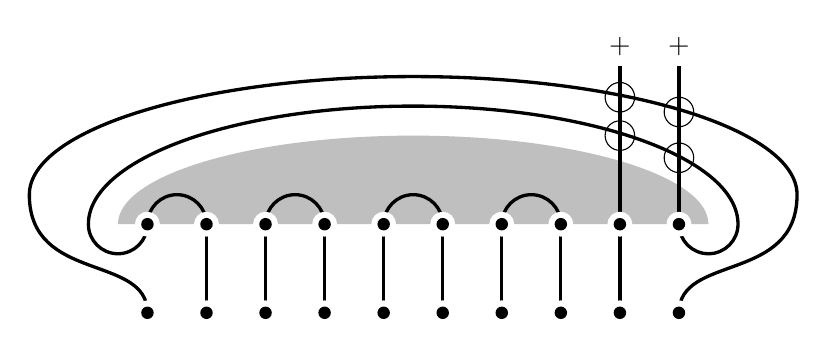
\begin{tikzpicture}[xscale=0.75,yscale=0.75]
	\foreach \x in {2,3,...,9}{
		\draw[very thick] (\x,0) -- (\x,-1.5);}
	\fill[black!25!white] (0.5,0) -- (10.5,0) arc (0:180:5cm and 1.5cm);
	\foreach \x in {1,3,...,7}{
		\draw[very thick] (\x,0) arc (180:0:0.5cm);}
	\draw[very thick] (9,0) -- (9,2.675) node[above] {+};
	\draw[very thick] (10,0) -- (10,2.675) node[above] {+};
	\draw[very thick] (1,0) arc (360:180:0.5cm) arc (180:0:5.5cm and 2cm) arc (360:180:0.5cm);
	\draw[very thick] (1,-1.5) .. controls (1,-0.5) and (-1,-1) .. (-1,0.5) arc (180:0:6.5cm and 2cm) .. controls (12,-1) and (10,-0.5) .. (10,-1.5);
	\foreach \x in {1,...,10} {
		\fill[white] (\x,0) circle (6pt);
		\fill (\x,0) circle (3pt);
		\fill[white] (\x,-1.5) circle (6pt);
		\fill (\x,-1.5) circle (3pt);}
	\draw[thin] (9,1.5) circle (0.25cm);
	\draw[thin] (10,1.125) circle (0.25cm);
	\draw[thin] (9,2.15) circle (0.25cm);
	\draw[thin] (10,1.9) circle (0.25cm);
\end{tikzpicture}
\end{split}
\end{equation*}

But if one restricts to singlet state vectors as the basis elements for the matrix entries
then this problem is bypassed.
In a spin singlet all the spin sites on the top row are paired together in a non-crossing
perfect matching. In particular there are no free strands extending to the top edge of the diagram
(or spanning from the top row to the bottom row in some conventions).
Then one may join left to right by a Temperley-Lieb generator without any crossings.
But this only works for the spin-singlet sector.

An example of a calculation is shown to demonstrate this point:
it shows the result of appling $-h^{\mathrm{FM}}_{L,1}$ to a particular Hulthen
bracket basis element, using the diagrammatic representation
\begin{equation*}
\begin{split}
&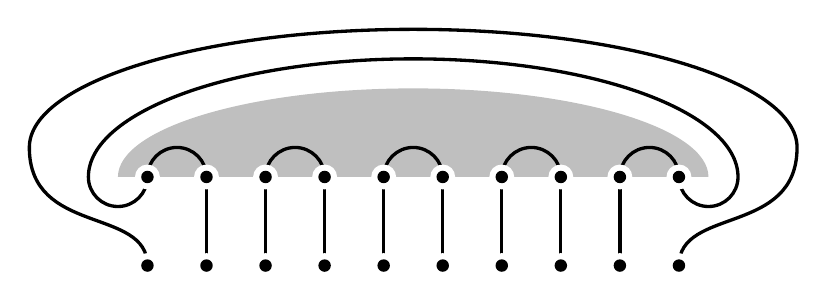
\begin{tikzpicture}[xscale=0.75,yscale=0.75]
	\foreach \x in {2,3,...,9}{
		\draw[very thick] (\x,0) -- (\x,-1.5);}
	\fill[black!25!white] (0.5,0) -- (10.5,0) arc (0:180:5cm and 1.5cm);
	\foreach \x in {1,3,...,9}{
		\draw[very thick] (\x,0) arc (180:0:0.5cm);}
	\draw[very thick] (1,0) arc (360:180:0.5cm) arc (180:0:5.5cm and 2cm) arc (360:180:0.5cm);
	\draw[very thick] (1,-1.5) .. controls (1,-0.5) and (-1,-1) .. (-1,0.5) arc (180:0:6.5cm and 2cm) .. controls (12,-1) and (10,-0.5) .. (10,-1.5);
	\foreach \x in {1,...,10} {
		\fill[white] (\x,0) circle (6pt);
		\fill (\x,0) circle (3pt);
		\fill[white] (\x,-1.5) circle (6pt);
		\fill (\x,-1.5) circle (3pt);}
\end{tikzpicture}\\[10pt]
&\hspace{3cm} =\,
\raisebox{0.5cm}{
\begin{minipage}{8cm}
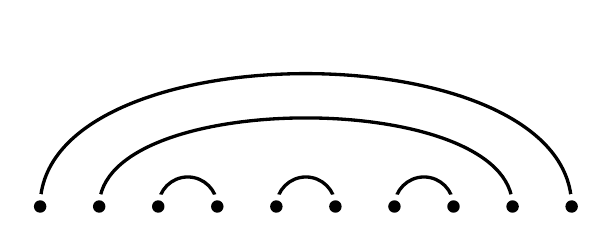
\begin{tikzpicture}[xscale=0.75,yscale=0.75]
%	\foreach \x in {2,3,...,9}{
%		\draw[very thick] (\x,0) -- (\x,-1.5);}
%	\fill[black!35!white] (0.5,0) -- (10.5,0) arc (0:180:5cm and 1.5cm);
	\foreach \x in {3,5,7}{
		\draw[very thick] (\x,0) arc (180:0:0.5cm);}
	\draw[very thick] (2,0) .. controls (2,2) and (9,2) .. (9,0);
	\draw[very thick] (1,0) .. controls (1,3) and (10,3) .. (10,0);
	\foreach \x in {1,...,10} {
		\fill[white] (\x,0) circle (6pt);
		\fill (\x,0) circle (3pt);}
\end{tikzpicture}
\end{minipage}}
\end{split}
\end{equation*}
No matter how one pairs up the spins in the grey region into any non-crossing perfect matching,
the resulting diagram will either be: 
another different Hulthen bracket basis vector, with coefficient 1;
or else a ``bubble'' resulting in a negative coefficient $-2$ but with the same
diagrammatric basis element, yielding a contribution to a diagonal matrix element
(which is allowed to be negative in the Perron-Frobenius theorem).
So all off-diagonal matrix entries are positive in the Hulthen bracket basis for the negative
of the Hamiltonian. So the Perron-Frobenius theorem applies.


The point of Lemma \ref{lem:first} is to demonstrate a symmetry property, namely non-degeneracy with respect to $H^{\mathrm{FM}}_{L}$.
That is not present in the other total spin sectors.
In order to see how this may be applied, note the following symmetry of the Hamiltonian
$$
\mathcal{R} : \Hil_{[1,L]} \to \Hil_{[1,L]}
$$
defined by linearly extending the prescription
$$
	\mathcal{R} (\psi_1 \otimes \psi_2 \otimes \cdots \otimes \psi_{L-1} \otimes
\psi_L)\, =\, \psi_{L} \otimes \psi_{L-1} \otimes \cdots \otimes \psi_2 \otimes \psi_1\, .
$$
In other words, this is reflecting in the ``pair of planes'' $0$ and $L/2$.
(See for example, \cite{DLS} for the notation.)
Also, let spin-flip symmetry be $\mathcal{F} = \exp(i \pi S_{[1,L]}^{(1)})$,
which is clearly a symmetry of the Hamiltonian.
Then, finally, let us define the momentum-$\ell$ spin raising- and lowering-operators
\begin{equation*}
	\widehat{S}^{\pm}_\ell\, =\, \sum_{\alpha=1}^{L} e^{2 \pi i \ell \alpha/L} S_{\alpha}^{\pm}\, ,
\end{equation*}
for $\ell \in \Z$.
Then
$$
\left(\widehat{S}^{+}_{\ell}\right)^*\, =\, \widehat{S}^-_{-\ell}\, .
$$
But also
$$
\widehat{S}^{-}_{-\ell}\, =\, \mathcal{R} \mathcal{F} \widehat{S}^{+}_{\ell}
\mathcal{F}\mathcal{R}\, .
$$
So the following corollary is applicable.
\begin{cor}
Suppose that $A$ is an operator on $\Hil_{[1,L]}$ such that there is some unitary operator
$U$ on $\Hil_{[1,L]}$, satisfying
\begin{itemize}
\item $A^*=U^*AU$, the unitary implements the adjoint for $A$,
\item $H^{\mathrm{FM}}_L = U^* H^{\mathrm{FM}}_L U$, $U$ is a symmetry of $H^{\mathrm{FM}}_{L}$,
\item $\mathcal{C}_{[1,L]} = U^* \mathcal{C}_{[1,L]} U$, $U$ commutes with
the Casimir operator.
\end{itemize}
Then we have the double-commutator formula for the first-order perturbation term:
$$
\langle \Psi_L^{(0)}\, ,\ A^* 
\big(H_{L}^{\mathrm{FM}}-E^{\mathrm{FM}}_{\min}(0;L)\big)
A \Psi_L^{(0)}\rangle\, 
=\, \frac{1}{2}\, \langle \Psi_L^{(0)}\, ,\ [A^*,[H_L^{\mathrm{FM}},A]] \Psi_L^{(0)}\rangle\, .
$$
\end{cor}
\begin{remark}
The single-mode-approximation consists of calculating the terms 
$$
\langle \Psi_L^{(0)}\, ,\ \widehat{S}^{-}_{-\ell} 
\big(H_{L}^{\mathrm{FM}}-E^{\mathrm{FM}}_{\min}(0;L)\big)
\widehat{S}^+_{\ell} \Psi_L^{(0)}\rangle\, .
$$
For example, see Chapter 9 from the textbook by Assa Auerbach \cite{Auerbach}.
\end{remark}
\begin{proof}
Because of the properties $U\Psi_L^{(0)}$ is an eigenvector of 
$H^{\mathrm{FM}}_{L}$ with eigenvalue 
$E^{\mathrm{FM}}_{\min}(0;L)$, which is in $\Hil_{[1,L]}^{(0)}$.
Therefore, by Lemma \ref{lem:first}, we have 
$U \Psi_{L}^{(0)} = e^{i \theta} \Psi_L^{(0)}$ for some $\theta \in \R$.
Thus,
\begin{equation*}
\begin{split}
	\langle \Psi_L^{(0)}\, ,\ A \big(H^{\mathrm{FM}}_{L}
	-E^{\mathrm{FM}}_{\min}(0;L)\big) A^* \Psi_L^{(0)}\rangle\,
	=\,
	\langle \Psi_L^{(0)}\, ,\ U^* A^* \big(H^{\mathrm{FM}}_{L}
	-E^{\mathrm{FM}}_{\min}(0;L)\big) A U \Psi_L^{(0)}\rangle\\
	=\, 	\langle \Psi_L^{(0)}\, ,\ A^* \big(H^{\mathrm{FM}}_{L}
	-E^{\mathrm{FM}}_{\min}(0;L)\big) A \Psi_L^{(0)}\rangle\,
\end{split}
\end{equation*}
But a trivial calculation shows that 
\begin{equation*}
\begin{split}
	\left\langle \Psi_L^{(0)}\, ,\ \left[A^*\, ,\ \left[\big(H^{\mathrm{FM}}_{L}
	-E^{\mathrm{FM}}_{\min}(0;L)\big)\, ,\ A\right]\right] 
	\Psi_L^{(0)}\right\rangle\,
	&=\,
	\langle \Psi_L^{(0)}\, ,\ A \big(H^{\mathrm{FM}}_{L}
	-E^{\mathrm{FM}}_{\min}(0;L)\big) A^* \Psi_L^{(0)}\rangle\\
	&\qquad+	\langle \Psi_L^{(0)}\, ,\ A^* \big(H^{\mathrm{FM}}_{L}
	-E^{\mathrm{FM}}_{\min}(0;L)\big) A \Psi_L^{(0)}\rangle\, ,
\end{split}
\end{equation*}
owing to the fact that $H^{\mathrm{FM}}_{L}
	-E^{\mathrm{FM}}_{\min}(0;L)$ annihilates $\Psi_L^{(0)}$.
Therefore, this proves the corollary because $[A^*,[H-c\mathbbm{1},A]]$
is independent of $c$.
\end{proof}
As we mentioned before, the single mode approximation (SMA)
is a popular perturbation scheme which is used because of its
ease of calculation.
We note that a standard exercise shows that, for $q_L=e^{2\pi i/L}$:
\begin{equation}
\label{eq:DoubleCommFinal}
\left[\widehat{S}_{-\ell}^-,  \left[\widehat{S}_{\ell}^+,H_{L}^{\mathrm{FM}}\right]\right]\,
	=\,  -\sum_{\alpha=1}^{L} \Big(2(1-q_L^\ell)(1-q_L^{-\ell}) S_\alpha^{(3)} S_{\alpha+1}^{(3)} 
+(1-q_L^\ell) S_\alpha^- S_{\alpha+1}^+
+(1-q_L^{-\ell})S_\alpha^+ S_{\alpha+1}^{-}\Big)\, .
\end{equation}
Then, defining the translation operator $\mathcal{T} : \Hil_{[1,L]} \to \Hil_{[1,L]}$, by linearly extending the prescription
$$
	\mathcal{T} (\psi_1 \otimes \psi_2 \otimes \psi_3 \otimes \cdots 
\otimes \psi_{L-1} \otimes \psi_L)\,
	=\, \psi_L \otimes \psi_1 \otimes \psi_2 \otimes \cdots \otimes \psi_{L-2}
\otimes \psi_{L-1}\, ,
$$
we also have $\mathcal{T} \Psi_L^{(0)} = e^{i\theta} \Psi_L^{(0)}$
for some $\theta$.
Using this, another exercise then shows that 
\begin{equation}
\label{eq:DoubleToDo2}
	\left\langle \Psi^{\mathrm{FM}}_{\min}(0;L)\, ,\  \widehat{S}_{-\ell}^- \left(H_{L}^{\mathrm{FM}}-E^{\mathrm{FM}}_{\min}(0;L)\right)\widehat{S}_{\ell}^+ 
 \Psi^{\mathrm{FM}}_{\min}(0;L)\right\rangle\, 
=\, \frac{8}{3}\, \sin^2\left(\frac{\pi \ell}{L}\right)\, 
\left(\frac{L}{4} - E^{\mathrm{FM}}_{\min}(0;L)\right)\, ,
\end{equation}
assuming normalization $\|\Psi^{\mathrm{FM}}_{\min}(0;L)\|=1$.
We will leave these exercises to the reader.
(You may see an earlier preprint version of this article available
on the arXiv, where full details are provided.)

It is easy to see that $E^{\mathrm{FM}}_{\min}(0;L)<L/4$
for even values of $L$ greater than $4$, numerically.
It can also be proved theoretically for sufficiently large $L$.
(See an earlier preprint version of
this article on the arXiv for full details.)
Therefore, we have the following result:
\begin{cor}
\label{cor:main}
Assuming that $L$ is even, we have
\begin{equation*}
E^{\mathrm{FM}}_{\min}(1;L)-E^{\mathrm{FM}}_{\min}(0;L)\, \leq\,
\mathcal{E}^{\mathrm{SMA}}_{\min}(0;L)\, ,
\end{equation*}
where $\mathcal{E}^{\mathrm{SMA}}_{\min}(0;L)$ is the single mode approximation
$$ 
\mathcal{E}^{\mathrm{SMA}}_{\min}(0;L)\,
=\, \min_{\ell=1,\dots,L-1}
\frac{\left\langle \Psi^{\mathrm{FM}}_{\min}(0;L)\, ,\ 
\widehat{S}^-_{-\ell} \left(H^{\mathrm{FM}}_{L}
-E^{\mathrm{FM}}_{\min}(0;L)\right) \widehat{S}^+_{\ell} \Psi^{\mathrm{FM}}_{\min}(0;L)\right\rangle}
{\left\|\widehat{S}^+_{\ell} \Psi^{\mathrm{FM}}_{\min}(0;L)\right\|^2}\, .
$$
In particular $\mathcal{E}^{\mathrm{SMA}}_{\min}(0;L)$ is positive
whenever $E^{\mathrm{FM}}_{\min}(0;L)<L/4$.
\end{cor}
By equation (\ref{eq:DoubleToDo2}), we have
$\mathcal{E}_{\min}^{\mathrm{SMA}}(0;L) = \min_{\ell=1,\dots,L-1}
\mathcal{E}_{\ell}^{\mathrm{SMA}}(0;L)$
where
$$
\mathcal{E}_{\ell}^{\mathrm{SMA}}(0;L)\, =\, 
\frac{8}{3}\, 
\left(\frac{L}{4} - E^{\mathrm{FM}}_{\min}(0;L)\right)\,
\frac{\sin^2\left(\pi \ell/L\right)}{\left\|\widehat{S}^+_{\ell} \Psi^{\mathrm{FM}}_{\min}(0;L)\right\|^2}\, .
$$
The denominator is clearly positive. We plot a numerical calculation of it
for an example $L=20$ in Figure \ref{fig:StructureFactor}.
% Figure environment removed
It is numerically evident that 
$1/\|\widehat{S}^+_{\ell}\Psi^{\mathrm{FM}}(0;20)\|^2$
is minimized (among $\ell=1,\dots,L-1$ modulo $L$) when $\ell=\pm 1$.
Hence, the SMA minimum is attained at $\ell=\pm 1$ because the same
is true of $\sin^2(\pi\ell/L)$.

For those practitioners who use the SMA, they usually assume that not
only does it provide a variational upper bound on the gap
$$
E^{\mathrm{FM}}_{\min}(1;L)-E^{\mathrm{FM}}_{\min}(0;L)\, ,
$$
as in Corollary \ref{cor:main}, but that the Rayleigh quotient
may actually give a good estimate of the gap.
We believe that the SMA is almost exactly 4 times too large in this context,
but the 2-mode approximation gives a much better bound, 
asymptotically exact.
This guess is based on numerical evidence.



\section{Review of known results: Sutherland}
In \cite{Sutherland}, Bill Sutherland analyzed $E^{\mathrm{FM}}_{\min}(S;L)$ using the Bethe ansatz.
Sutherland claimed that he had proved weak paramagnetism.
We have carried out numerical analysis up to $L=20$ and we see evidence
for the following. (See Figure \ref{fig:GSEtable}.)
\begin{itemize}
\item For $L\geq 4$ we have 
$E^{\mathrm{FM}}_{\min}(1;L)>E^{\mathrm{FM}}_{\min}(0;L)$.
But for no $L$ do we have 
$E^{\mathrm{FM}}_{\min}(S+1;L)>E^{\mathrm{FM}}_{\min}(S;L)$
for any $S>0$.
\end{itemize}
One may call this ``weak paramagnetism'' at the spin singlet.
It is paramagnetism because the energy of the lower spin $S=0$
is lower than the energy of the higher spin $S=1$, despite the fact that
the model is generally ferromagnetic otherwise.

But Sutherland appears to have meant something different by his
term ``weak paramagnetism.''
Sutherland claims that, in terms of complete
elliptic integrals of the first and second kind,
\begin{equation}
\begin{split}
	d\, &=\, \frac{1}{2} - \frac{a}{2}\, \left(1-\frac{E(1/a)}{K(1/a)}\right)\, ,\\
	\varepsilon\, &=\, 4 K\left(\frac{1}{a}\right)\left(2 E\left(\frac{1}{a}\right) - \left(1-\frac{1}{a^2}\right)K\left(\frac{1}{a}\right)\right)\, ,
\end{split}
\end{equation}
where $\varepsilon = 2 E^{\mathrm{FM}}_{\min}(S;L)/L$
and $d=\frac{1}{2}-\frac{S}{L} \in [0,1/2]$.
Using the regular parametrization of the complete elliptic integrals,
one obtains
$$
	\varepsilon\, =\, \pi^2\left(1+8\left(d-\frac{1}{2}\right)^2\right) + 
O\left(\left(d-\frac{1}{2}\right)^4\right)\ \text{ as $d \to \frac{1}{2}^-$.}
$$
This is what is found by standard calculations and this is what is claimed
by Sutherland. He claims that this implies weak paramagnetism.
But, unfortunately, both the functions $d$ and $\varepsilon$ are monotone 
in $a$, meaning that this formula would imply complete {\em antiferromagnetism}, which is definitely incorrect.
The absolute ground state of the ferromagnet is the spin $S=L/2$ eigenstate
$\Psi_{\min}^{\mathrm{FM}}(L/2;L)$; it is {\em not} the spin singlet.

It is interesting that if one uses an unusual parametrization of the complete
elliptic integrals, the parametrization used in Wolfram Mathematica,
then there is a turn-around. But even then the sign is wrong.
Moreover, that parametrization does not conform to Sutherland's asymptotic
formula above. (So we doubt that the Mathematica parametrization
was Sutherland's meaning.)

We note that the underlying idea of Sutherland's approach seems sound.
The Bethe ansatz roots develop a violation of the string hypothesis
where the roots accumulate along certain curves, to be determined, with
certain densities.
These are examples of singular integral equations, which may be
transformed into the type that is solved by complete elliptic integrals.
But we believe that the final steps of Sutherland's presentation are in 
error, and no further clarification exists in the literature.



% Figure environment removed


\subsection{Review of known results: Dhar and Shastry}

In \cite{DharShastry}, Dhar and Shastry reconsidered the problem originally considered by Sutherland, and showed that the Bethe ansatz equations
for these vectors reduce to a 1-parameter generalization of the Stieltes equations familiar from solving for roots
of orthogonal polynomials.
The advantage is that their equations are explicitly algebraically solvable rational equations; whereas, the Bethe ansatz equations are transcendental integrable systems.
In addition they posited that the vectors  may be written as 
$\Psi^{\mathrm{FM}}_{\min}(S;L)\, =\, \Xi_{L}^{\mathrm{Bloch}}(S)$ where
\begin{equation*}
	\Xi_{L}^{\mathrm{Bloch}}(S)\, =\, \left(\widehat{S}^{-}_{1}\right)^{(L/2)-S} \Big(\Psi_{1/2,1/2} \otimes \cdots \otimes \Psi_{1/2,1/2}\Big)\, .
\end{equation*}
or else $\overline{\Xi}_{L}^{\mathrm{Bloch}}(S)$ which is 
$\mathcal{R} \Xi_{L}^{\mathrm{Bloch}}(S) \mathcal{R}$.
They call these Bloch walls. 

They argued that the limiting form of the energies are 
\begin{equation*}
	E^{\mathrm{FM}}_{\min}(S;j,L)\, \sim\, \frac{2\pi^2}{L}\, \cdot \left(j^2-\frac{S^2}{L^2}\right)\, ,
	\text{ as $L \to \infty$.}
\end{equation*}
One can check from  Figure \ref{fig:BlochWallApprox} that this is close to the exact formula for $L=20$.

\begin{remark}
An interesting point is that for the spin $1/2$  XXZ spin ring with Ising like anisotropy,
\begin{equation*}
H_{[1,L]}^{(q)}\, =\, \sum_{\alpha=1}^{L} \left(\frac{1}{4}\, \mathbbm{1} - S^{(3)}_{\alpha} S^{(3)}_{\alpha+1}
-\frac{2}{q+q^{-1}}\left(S^{(1)}_{\alpha}S^{(1)}_{\alpha+1} + S^{(2)}_{\alpha} S^{(2)}_{\alpha+1}\right)\right)\, ,
\end{equation*}
with $0\leq q\leq 1$, it is known that the elementary excitations are literal droplets
of spin, with both a left and right domain wall, asymptotically when $L \to \infty$. See \cite{NachtergaeleStarrDroplet}.
Moreover, there is a closely related $\mathrm{SU}_q(2)$-symmetric version of the XXZ chain with kink or anti-kink
boundary conditions, where the droplets are still the elementary excitations, apparently created by introducing 
an interface of the opposite type: a droplet consists of both a kink and anti-kink interface at the left and right domain walls.
See \cite{NSSdroplet}.
\end{remark}

There are challenges in Dhar and Shastry's approximation, as well.
Primarily, even at $S=0$, they find two distinct Bloch walls,
$\Xi_{L}^{\mathrm{Bloch}}(0)$ and 
$\overline{\Xi}_{L}^{\mathrm{Bloch}}(0)$.
Neither vector is real.
But Lemma \ref{lem:first} implies that the lowest energy spin singlet
is non-degenerate.
Therefore, Dhar and Shastry's formula must break down as an approximation
at $S=0$.
Indeed this is what Figure \ref{fig:BlochWallApprox} shows.

% Figure environment removed
Setting $K=\frac{1}{2}L-S$, and letting $\Omega_L = \Psi_{1/2,1/2} \otimes 
\cdots \otimes \Psi_{1/2,1/2}$ (with $L$ tensor factors),
\begin{equation*}
\begin{split}
	\langle \overline{\Xi}_{L}^{\mathrm{Bloch}}(S)\, ,\ 
\Xi_{L}^{\mathrm{Bloch}}(S)\rangle\,
	&=\, (K!)^2 \sum_{\substack{1\leq x(1)<\dots<x(K)\leq L\\
1\leq y(1)<\dots<y(K)\leq L}}
q_L^{x(1)+\dots+x(K)} q_L^{y(1)+\dots+y(K)}\\
&\hspace{2cm} \cdot \langle (S_{x(1)}^- \cdots S_{x(K)}^-)\Omega_L\, ,\
(S_{y(1)}^- \cdots S_{y(K)}^-)\Omega_L\rangle\, ,
\end{split}
\end{equation*}
where, as before, $q_L = e^{2\pi i/L}$.
The final inner-product inside the summation on the right-hand-side
is non-zero if and only if $x(k)=y(k)$ for all $k \in \{1,\dots,K\}$.
Therefore, we obtain the $q$-binomial
\begin{equation*}
	\langle \overline{\Xi}_{L}^{\mathrm{Bloch}}(S)\, ,\ 
\Xi_{L}^{\mathrm{Bloch}}(S)\rangle\,
	=\, (K!)^2 
\left[\begin{matrix}L \\ K\end{matrix}\right]_{q^2} q^{K(K+1)} \Bigg|_{\substack{q=q_L\\K=(L/2)-S}}\, .
\end{equation*}
By the same calculation,
\begin{equation*}
	\|\overline{\Xi}_{L}^{\mathrm{Bloch}}(S)\|^2\, =\, 
\|\Xi_{L}^{\mathrm{Bloch}}(S)\|^2\,
	=\, (K!)^2 \binom{L}{K}\Bigg|_{K=(L/2)-S}\, .
\end{equation*}
Since $q=q_L$ is a root-of-unity, the $q$-Lucas theorem applies, for example from \cite{KlugeRubey} Lemma 3.1,
$$
\left[\begin{matrix}L \\ K\end{matrix}\right]_{q^2}\, =\, \binom{\lfloor L/R \rfloor}{\lfloor K/R \rfloor}\cdot
\left[\begin{matrix}L - R \lfloor L/R \rfloor\\ K - R\lfloor K/R \rfloor \end{matrix}\right]_{q^2}\, ,\
\text{ for }\ R=\min(\{r \in \{1,2,\dots\}\, :\, q^{2r}=1\})\, .
$$
Note that for $q=q_L$, we have $R=L/2$.
If $K<R$ then the inner-product turns out to be $0$ because $[L]_{q^2}!/[L-K]_{q^2}!$ has a factor $[L]_{q^2}$ which is 0
(since $q^{2L}=0$) but $[K]_{q^2}!$ is not $0$. This is also necessitated by consideration of translation eigenvalues.

If $K=R=L/2$ then the $q$-binomial coefficient on the right-hand-side of the formula above equals 1.
So the inner product is exactly $2(K!)^2$.
But the norm-squared of each vector is $\binom{L}{L/2} (K!)^2$.
This means that the cosine of the angle between the two vectors
is approximately $2^{-L+1}\sqrt{\pi L/2}$.
The two vectors are nearly orthogonal.
Therefore, if one takes Dhar and Shastry's approximation
seriously, one obtains two ground states in the spin singlet
sector.
But Lemma \ref{lem:first} proves that the ground state is unique.

In order to help understand the term $1/\|\widehat{S}_{\ell}^+ \Psi^{\mathrm{FM}}_{\min}(0;L)\|^2$, let us cite the results
for Dhar and Shastry's ``Bloch wall'' states.
It is approximately as simple to calculate the structure factor in the pure Bloch wall ansatz 
as it is to calculate the inner-product of two Bloch wall vectors.
We leave this as an exercise to the interested reader.
(Complete details of the calculation are included in an earlier preprint
version on the arXiv.)
We have 
\begin{equation*}
\frac{\|\widehat{S}^+_{\ell}\cdot \Xi_{L}^{\mathrm{Bloch}}(0;L)\|^2}{\|\Xi_{L}^{\mathrm{Bloch}}(0;L)\|^2}\, 
=\, \begin{cases} (L/2) ((L/2)+1) & \text{ if $\ell\equiv -1\ (\operatorname{mod} L)$,}\\
(L/2)((L/2)-1)/(L-1)& \text{ if $\ell\not\equiv -1\ (\operatorname{mod} L)$.}
\end{cases}
\end{equation*}
This verifies the necessary identity 
$$
\sum_{\ell=1}^L\frac{\|\widehat{S}^+_{\ell}\cdot \Xi_{L}^{\mathrm{Bloch}}(0;L)\|^2}{\|\Xi_{L}^{\mathrm{Bloch}}(0;L)\|^2}\,
=\, \frac{1}{2}\, L^2\, .
$$
%
%However, in term of the energy expectation, we get
%$$
%\sum_{m=1}^{L} \cos\left(\frac{2\pi m}{L}\right) \frac{\|\widehat{S}^+_{m}\cdot \Xi_{\ell}(0;1/2,L)\|^2}{\|\Xi_{\ell}(0;1/2,L)\|^2}\,  =\, \cos\left(-\frac{2\pi \ell}{L}\right) \left(\frac{L}{2}\left(\frac{L}{2}+1\right) - \frac{(L/2)((L/2)-1)}{L-1}\right)
%$$
%This equals $\cos(2\pi \ell/L) L^3 /(4L-4)$. If we recall that this is supposed to equal $(2L/3) (-E^{\mathrm{FM}}_{\min}(0;j,L)+j^2L)$ (for $j=1/2$) this would give that the variational energy of the pure Bloch wave is approximately $L^2/12$.
%But this is not numerically verified. 
%Dhar and Shastry's formula, $(2\pi^2/L) (j^2 - \frac{S^2}{L^2})$, which seems to be quite a good approximation,
%gives $E^{\mathrm{FM}}_{\min}(0;j,L) \sim \pi^2/(2L)$ for $j=1/2$ and $L \to \infty$.

Finally if we take $\ell =0$, and we apply spin-flip symmetry,
we can see that the expectation of the Casimir operator in the state given by the vector 
$\Xi_{L}^{\mathrm{Bloch}}(0;L)$
is $\sim L/4$. 
This also shows the limitation of the Bloch wall approximations because
the total spin should be $0$.
The formula 
$$
\sum_{\ell=1}^{L} \cos\left(\frac{2\pi \ell}{L}\right) 
\frac{\|\widehat{S}^+_{\ell}\cdot \Xi_{L}^{\mathrm{Bloch}}(0;L)\|^2}{\|\Xi_{L}^{\mathrm{Bloch}}(0;L)\|^2}\,  =\, \cos\left(-\frac{2\pi }{L}\right) \left(\frac{L}{2}\left(\frac{L}{2}+1\right) - \frac{(L/2)((L/2)-1)}{L-1}\right)\, ,
$$
is equal to
$L(-E^{\mathrm{FM}}_{\min}(0;L)+j^2L)+L(L/(4(L-1)))$ 
because the Bloch wall expectation of $\sum_{x=1}^{L} S_x^{(3)} S_{x+1}^{(3)}$
is equal to $-L/(4(L-1))$.
Thus, if we assume that the Bloch wall states are exact
instead of just approximations, this would give
$E^{\mathrm{FM}}_{\min}(0;L) \sim \pi^2/(2L)$ as $L \to \infty$.
This is also what Dhar and Shastry's formula gives 
$(2\pi^2/L) (j^2 - \frac{S^2}{L^2})$ for  $S=0$.
This seems to be quite a good approximation.
But it does overestimate the numerically obtained formulas slightly.
See for instance Figure \ref{fig:BlochWallApprox}.
So one does need a correction to the pure Bloch wall if one wants to correct the energy downward.

\begin{remark} Let us write $\mathcal{Z}(0;L) = \left\|\widehat{S}^+_{\ell} \Psi^{\mathrm{FM}}_{\min}(0;L)\right\|^2$, where we assume $\left\| \Psi^{\mathrm{FM}}_{\min}(0;L)\right\|^2=1$.
According to the numerical figure,
Figure \ref{fig:StructureFactor},
 we may see that one possibility is $\mathcal{Z}(\ell;L) \approx \frac{L}{3} + \frac{L^2}{12} \left(\delta_{\ell,1}+\delta_{\ell,-1}\right)$.
This is not exactly right because $\mathcal{Z}(0;L)=0$ since $\widehat{S}^+_0 \Psi^{\mathrm{FM}}_{\min}(0)$
equals  $0$ by $\mathrm{SU}(2)$ symmetry (the singlet property).
But that is a lower-order correction. If we took it into account, we might guess that
$\mathcal{Z}(\ell;L) \approx \frac{L}{3} \big(1-\delta_{\ell,0}-\delta_{\ell,1}-\delta_{\ell,-1}\big) 
+ \frac{L(L+6)}{12} \big(\delta_{\ell,1}+\delta_{\ell,-1}\big)$.
\end{remark}

\section{Additional numerics and mathematical physics motivation}

It is frequently believed that the single mode approximation
gives insight to the actual energy gap.
We find numerically that the SMA is approximately 4 times too large.
See Figure
\ref{fig:DataAn}.
% Figure environment removed
We do not have a theoretical explanation.
But further numerical investigation which we do not report on here
suggests to us that the 2-mode approximation is much
sharper.
(We believe that the 2-mode approximation is asymptotically sharp
for this purpose.)


\subsection{Implication for Ferromagnet Ordering of Energy Levels}
\label{subsec:FOEL}


The notion of ferromagnetic ordering of energy levels is based on the Lieb-Mattis theorem of, ``Ordering of Energy Levels,'' from \cite{LiebMattisOEL}.
The Lieb-Mattis theorem for antiferromagnets (and ferrimagnets) says the following.
Defining the minimum energies in the total spin spaces as
\begin{equation*}
	E_{\min}^{\mathrm{AF}}(S;j,L)\, =\, \min\left(\left\{\frac{\langle \psi\, ,\ H_{j,L}^{\mathrm{AF}} \psi \rangle}{\|\psi\|^2}\, :\, 
	\psi \in \Hil_{[1,L]}^{(j)}\, ,\ \|\psi\|\neq 0\, ,\ \mathcal{C}_{\mathrm{tot}} \psi = S(S+1) \psi\right\}\right)\, .
\end{equation*}
Lieb and Mattis proved the following: the ground state is non-degenerate and
\begin{equation*}
E_{\min}^{\mathrm{AF}}(0;j,L)\, 
<\, E_{\min}^{\mathrm{AF}}(1;j,L)\,
<\, E_{\min}^{\mathrm{AF}}(2;j,L)\,
<\, \dots\, 
<\, E_{\min}^{\mathrm{AF}}(jL;j,L)\, ,
\end{equation*}
and their theorem applies equally well to any connected, bipartite, balanced graph.

For the ferromagnet, the Perron-Frobenius theorem implies $E_{\min}^{\mathrm{FM}}(jL;j,L)$ is less than
$E_{\min}^{\mathrm{FM}}(S;j,L)$ for all $S<jL$.
Caputo, Liggett and Richthammer proved in \cite{CaputoLiggettRichthammer} a result implying
\begin{equation*}
	E_{\min}^{\mathrm{FM}}(jL-1;j,L)\, =\, \min(\{E_{\min}^{\mathrm{FM}}(S;j,L)\, :\, S=0,1,\dots,jL-1\})\, ,
\end{equation*}
and that the analogous result holds for any connected graph.
In \cite{NSSfoel}, the property of FOEL-$n$, or ``ferromagnetic ordering of energy levels at order $n$,''
is defined as follows: for all $m\leq n$ we have
\begin{equation*}
\forall \ell \in \{m+1,m+2,\dots,\lfloor jL\rfloor\}\, ,\ \text{ we have }\
	E_{\min}^{\mathrm{FM}}(jL-m;j,L)\, \leq\, E_{\min}^{\mathrm{FM}}(jL-\ell;j,L)\, .
\end{equation*}
For open chains with spins $j=1/2$, this was proved in the same article.
Then it was proved for open chains for $j>1/2$ in \cite{NachtergaeleStarr}.
The key is the Hulth\'en bracket basis, which was most famously exposed by Temperley and Lieb \cite{TemperleyLieb}.


But for spin rings, it appears to be false that FOEL-$n$ holds for every $n$. In \cite{SpitzerStarrTran}, some numerical evidence was provided.
To us, the numerical evidence seems like the most reliable indication of what is true.
In the present article we have extended that numerical evidence.
Following Corollary \ref{cor:main} we see a heuristic explanation of why FOEL-$n$ is violated
for spin rings for $n=jL-1$. 

We note that in the present article we have restricted attention to 
spins $j=1/2$ for simplicity of presentation.
But in an earlier preprint version of this article on the arXiv we have
reported some numerical evidence and results for spins higher than $1/2$.

\begin{remark}
Originally, David Aldous conjectured that the spectral gap of the interchange process is the same as the spectral gap of the symmetric exclusion process and also the same as the spectral gap of the random walk.
(See, for instance, the early paper of Handjani and Jungreis \cite{HandjaniJungreis}.)
That implies FOEL-$1$, and  Caputo, Liggett and Richthammer proved the full Aldous conjecture.
Dieker also had important work related to that problem \cite{Dieker}.
Morris \cite{Morris} and also Conomos and Starr \cite{ConomosStarr} had previously proved asymptotic FOEL-$1$ on boxes.
\end{remark}

After the proof by Caputo, Liggett and Richthammer, it was argued that asymptotic FOEL holds for boxes in \cite{NachtergaeleSpitzerStarrPre}
by Nachtergaele, Spitzer and one of the authors.
This means that for sufficiently large boxes $\{1,\dots,L\}^d$, FOEL-$n$ holds, if $L\geq L_0(n)$,
for each $n$ (where the minimum $L$ value $L_0(n)$ is a function of $n$).
If one considers the interchange process, which may be considered to be a $\mathrm{SU}(n)$ model when $L=n$,
then Alon and Kozma \cite{AlonKozma} have proved many extra interesting inequalities in the ``Aldous ordering.''
Since this model projects onto the Heisenberg model and other $\mathrm{SU}(k)$ models, for $k\leq n$, their results have implications
for all lower projections of the interchange process.



\subsection{Review of some motivation from mathematical physics}

One motivation for all of this is the fact that in mathematical physics, the phase transition
for the quantum Heisenberg ferromagnet has not yet been proved, even though for the quantum Heisenberg
antiferromagnet it was proved by Dyson, Lieb and Simon \cite{DLS}.
Their method for the antiferromagnet was reflection positivity.
But that property does not hold for the quantum Heisenberg ferromagnet, as proved by Speer \cite{Speer}.
Later, Correggi, Giuliani and Seiringer did prove  the type of inequalities that one would expect from
linear spin wave analysis \cite{CGS}.
But, the phase transition for the quantum Heisenberg ferromagnet has still not been proved.
If one changes the model to add any small amount of Ising-like anisotropy it was proved by Tom Kennedy \cite{Kennedy},
but that model has $\mathrm{U}(1)$ symmetry instead of $\mathrm{SU}(2)$.





%This is as much as we can say about $\mathcal{Z}(\ell;j,L)$ at present.
\section{Outlook and further results}

Two of the authors have begun to consider the 2-mode approximation in
collaboration with Wolfgang Spitzer.
This is closely related to spin wave theory.
The interesting property of spin wave theory is that linear spin wave
theory may be tested in terms of self-consistency if one considers
quadratic spin wave corrections.
We propose to do the similar approach for $n$-mode approximation.

We also hope to implement numerical improvements to our basic algorithm,
which is just the Lanzcos algorithm in Matlab.
For example, we wish to parallelize the calculation.
Another improvement would be to run the DMRG method or perhaps
a quantum Monte-Carlo algorithm.
For example, an old result using that method is \cite{GJL}.
We have begun working on the latter with Sardar Jaman, to whom
we are grateful for some insights already.

The SMA applied to the Bloch walls seems to lead to a self-consistent
theory.
This provides a particular perspective on the work that Dhar
and Shastry already accomplished on their own.
But there may be a possibility that within the 2-mode-approximation
an instability develops.
It would be interesting, if this occurs, to see where it occurs.

The most important problem remaining to us is to clarify Sutherland's approach.
His article seems to be at least 90\% correct.
But the way he reported some of his final results is confusing or in error.
This should be easy by now since there is such a well-developed
theory for the Bethe ansatz.
(See for example \cite{BKI} to start.)

In the appendix we provide the script for our Matlab code.
All data from our investigations is reported in this article.

\section*{Acknowledgments}

The authors gratefully acknowledge the resources provided by the University of Alabama at Birmingham IT-Research Computing group for high performance computing (HPC) support and CPU time on the Cheaha compute cluster.
S.S.~is grateful to Sardar Jaman for useful discussions.
This work was supported by a grant from the Simons Foundation.
Support provided by the National Aeronautics and Space Administration (NASA), Alabama Space Grant Consortium, Research Experiences for Undergraduates (REU) at UAB

\appendix


\section{The Matlab code Hulthen.m}

The following Matlab script implements the Hulth\'en bracket basis for calculating $E^{\mathrm{FM}}_{\min}(S;1/2,L)$ for each $S$.
We have written it for $L=20$ which is the largest length spin ring we could attain with our computing resources.

\scriptsize

\begin{verbatim}
E11 = sparse([1 0; 0 0]);
E12 = sparse([0 1; 0 0]);
E21 = sparse([0 0; 1 0]);
E22 = sparse([0 0; 0 1]);
h = kron(E11,E22)+kron(E22,E11)-kron(E12,E21)-kron(E21,E12);

L=20;
fileID = fopen('L20sparse.txt','a');

dim=2^L;

Adj = diag(ones(L-1,1),1);
Adj(1,L)=1;

H = sparse(dim,dim);
for x=1:(L-1)
    for y=(x+1):L
        if Adj(x,y)
            H=H+kron(speye(2^(x-1)),kron(E11,kron(speye(2^(y-x-1)),kron(E22,speye(2^(L-y))))));
            H=H+kron(speye(2^(x-1)),kron(E22,kron(speye(2^(y-x-1)),kron(E11,speye(2^(L-y))))));
            H=H-kron(speye(2^(x-1)),kron(E12,kron(speye(2^(y-x-1)),kron(E21,speye(2^(L-y))))));
            H=H-kron(speye(2^(x-1)),kron(E21,kron(speye(2^(y-x-1)),kron(E12,speye(2^(L-y))))));
        end
    end
end

% % Cas=zeros(2^L);
% Cas = sparse(dim,dim);
% for x=1:(L-1)
%     for y=(x+1):L
%         Cas=Cas+kron(speye(2^(x-1)),kron(E11,kron(speye(2^(y-x-1)),kron(E22,speye(2^(L-y))))));
%         Cas=Cas+kron(speye(2^(x-1)),kron(E22,kron(speye(2^(y-x-1)),kron(E11,speye(2^(L-y))))));
%         Cas=Cas-kron(speye(2^(x-1)),kron(E12,kron(speye(2^(y-x-1)),kron(E21,speye(2^(L-y))))));
%         Cas=Cas-kron(speye(2^(x-1)),kron(E21,kron(speye(2^(y-x-1)),kron(E12,speye(2^(L-y))))));
%     end
% end

DnSpinMat=[];
idxLst=[];
NumBracketLst=[];
for idx = 1:dim,
    base2rep = dec2base(idx-1,2);
    LengthBase2 = length(base2rep);
    DnSpinLst=[];
    for kctr=1:LengthBase2,
        if base2rep(kctr)=='1',
            DnSpinLst = [DnSpinLst,L-LengthBase2+kctr];
        end
    end
    if length(DnSpinLst)==L/2,
        idxLst=[idxLst,idx];
        DnSpinMat=[DnSpinMat;DnSpinLst];   
    end
end
%DnSpinMat
%idxLst
vectorLst=[];
for kctr=1:length(DnSpinMat)
    bracketLstLeft=[];
    bracketLstRight=[];
    for j=1:(L/2),
        if DnSpinMat(kctr,j)>j+length(bracketLstLeft),
            bracketLstRight=[bracketLstRight,DnSpinMat(kctr,j)];
            UpSpinCompatibleLst=setdiff(setdiff(1:DnSpinMat(kctr,j),DnSpinMat(kctr,1:j)),bracketLstLeft);
            bracketLstLeft=[bracketLstLeft,max(UpSpinCompatibleLst)];
        end
    end
%    [bracketLstLeft;bracketLstRight]
    NumBracketLst=[NumBracketLst,length(bracketLstLeft)];
    v = sparse(idxLst(kctr),1,1,dim,1);
    for j=1:length(bracketLstLeft),
        a=bracketLstLeft(j);
        b=bracketLstRight(j);
        v = v-kron(speye(2^(a-1)),kron(E21,kron(speye(2^(b-a-1)),kron(E12,speye(2^(L-b))))))*v;
    end
    ExcessDnSpin = setdiff(DnSpinMat(kctr,:),bracketLstRight);
    for j=1:length(ExcessDnSpin)
        a=ExcessDnSpin(j);
        v = kron(speye(2^(a-1)),kron(E12,speye(2^(L-a))))*v;
    end
    vectorLst = [vectorLst,v];
end

for numBrktCtr = 0:(L/2)
%    numBrktCtr
    fprintf(fileID,'%d\r\n\r\n',numBrktCtr);
    Indices = find(NumBracketLst==numBrktCtr);
    vMat = vectorLst(:,Indices);
    Amat = vMat'*H*vMat;
    Bmat = vMat'*vMat;
    E0 = eigs(Amat,Bmat,1,'smallestreal','Tolerance',1e-4);
    fprintf(fileID,'%f\r\n\r\n',E0);
end
fclose(fileID);
\end{verbatim}

\normalsize
To obtain the full eigenvalue list (for sufficiently small values of $L$ such as $L=12$, where this is feasible)
change the final for-loop to this:

\scriptsize

\begin{verbatim}

for numBrktCtr = 0:(L/2)
    numBrktCtr
    Indices = find(NumBracketLst==numBrktCtr);
    vMat = vectorLst(:,Indices);
    Amat = vMat'*H*vMat;
    Bmat = vMat'*vMat;
    [V,D] = eig(full(Amat),full(Bmat),'chol');
        fprintf(fileID,'%f\r\n\r\n',diag(D));
end
fclose(fileID);
end
\end{verbatim}

\normalsize
%
%\section{First commutator calculations}
%\label{app:FirstCommut}
%
%We first calculate
%\begin{equation}
%\label{eq:FirstComm}
%\begin{split}
%	\sum_{r'=1}^{L} [\widetilde{\mathcal{O}}_k^+,S_{r'}^{(3)} S_{r'+1}^{(3)}]\,
%	&=\,
%	\sum_{r=1}^{L} \sum_{r'=1}^{L} e^{2\pi i kr/L} [S_r^{+},S_{r'}^{(3)} S_{r'+1}^{(3)}]\\
%	&=\, \sum_{r=1}^{L} \sum_{r'=1}^{L} e^{2\pi i kr/L} \Big(  [S_r^{+},S_{r'}^{(3)}] S_{r'+1}^{(3)} 
%	+  S_{r'}^{(3)} [S_r^+,S_{r'+1}^{(3)}]\Big)\\
%	&=\, -\sum_{r=1}^{L} \sum_{r'=1}^{L} e^{2\pi i kr/L} \big(  \delta_{r,r'} S_r^+ S_{r'+1}^{(3)} 
%	+\delta_{r'+1,r}  S_{r'}^{(3)} S_r^+\big)\\ 
%	&=\, -\sum_{r=1}^{L}   \big( e^{2\pi i kr/L}  S_r^+ S_{r+1}^{(3)} 
%	+ e^{2\pi i (k+1)r/L} S_{r}^{(3)} S_{r+1}^+\big)\, .
%\end{split}
%\end{equation}
%Therefore, this implies
%\begin{equation}
%\begin{split}
%\label{eq:FirstCommPrime}
%	[\widetilde{\mathcal{O}}_k^+,H_L^{(Z)}]\,
%	=\,	
%	-\sum_{r=1}^{L} [\widetilde{\mathcal{O}}_k^+,S_{r}^{(3)} S_{r+1}^{(3)}]\,
%	=\, \sum_{r=1}^{L}   \big( e^{2\pi i kr/L}  S_r^+ S_{r+1}^{(3)} 
%	+ e^{2\pi i (k+1)r/L} S_{r}^{(3)} S_{r+1}^+\big)\, .
%\end{split}
%\end{equation}
%Now, let us turn our attention to $H_L^{(XY)}$.
%We note that
%we may also rewrite
%\begin{equation*}
%%\label{eq:HamiltonianFormulaXY2}
%	H_{L}^{(XY)}\,  =\, - \sum_{r=1}^{L} \Big(S_r^{(1)} S_{r+1}^{(1)} + S_r^{(2)} S_{r+1}^{(2)}\Big)\,
% =\, -\frac{1}{2}\, \sum_{r=1}^{L} \Big(S_r^{+} S_{r+1}^{-} + S_r^{-} S_{r+1}^{+}\Big)\, .
%\end{equation*}
%Because spin-raising operators commute with other spin-raising operators, we may write
%\begin{equation*}
%	[\widetilde{\mathcal{O}}_k^+,S_r^-S_{r+1}^+]\, =\, 	[\widetilde{\mathcal{O}}_k^+,S_r^-] S_{r+1}^+\, ,
%\end{equation*}
%which is $2e^{2\pi i k r/L} S_r^{(3)} S_{r+1}^-$.
%Then we get, by summing
%\begin{equation}
%\label{eq:HpmComm}
%	-\frac{1}{2}\, \sum_{r=1}^{L}  [\widetilde{\mathcal{O}}_k^+,S_{r}^{-} S_{r+1}^{+}]\,
%	=\, -\sum_{r=1}^{L} e^{2\pi i kr/L} S_r^{(3)} S_{r+1}^{+} \, .
%\end{equation}
%By a similar calculation,
%\begin{equation}
%\label{eq:HmpComm}
%	-\frac{1}{2}\, \sum_{r=1}^{L}  [\widetilde{\mathcal{O}}_k^+,S_{r}^{+} S_{r+1}^{-}]\,
%	=\, -\sum_{r=1}^{L} e^{2\pi i k(r+1)/L} S_r^{+} S_{r+1}^{(3)} \, .
%\end{equation}
%Therefore, adding equations (\ref{eq:HpmComm}) and (\ref{eq:HmpComm}), we have
%\begin{equation*}
%	 [\widetilde{\mathcal{O}}_k^+,H_L^{(XY)}]\,
%	=\, -\sum_{r=1}^{L} \big(e^{2\pi i kr/L} S_r^{(3)} S_{r+1}^{+} +
%	e^{2\pi i k(r+1)/L} S_r^{+} S_{r+1}^{(3)}\big)\, .
%\end{equation*}
%Together with (\ref{eq:FirstCommPrime}) this equation proves (\ref{eq:TBAapp1a}) and (\ref{eq:TBAapp1b}).
%
%\section{Double commutator in first order perturbation theory}
%\label{app:DoubleCommut}
%
%Since we have assumed $H_{j,L}^{\mathrm{FM}} \Psi = E \Psi$, or $(H_{j,L}^{\mathrm{FM}}-E \mathbbm{1}) \Psi = 0$, 
%and since $[H_{j,L}^{\mathrm{FM}}-E \mathbbm{1},\cdot]=[H_{j,L}^{\mathrm{FM}},\cdot]$,
%\begin{equation*}
%\langle \Psi\, ,\  \widetilde{\mathcal{O}}_{-k}^- (H_{j,L}^{\mathrm{FM}}-E) \widetilde{\mathcal{O}}_k^+ \Psi\rangle\, 
%=\, \langle \Psi\, ,\  \widetilde{\mathcal{O}}_{-k}^-  [H_{j,L}^{\mathrm{FM}},\widetilde{\mathcal{O}}_k^+] \Psi\rangle\, .
%\end{equation*}
%Then we may continue in this way
%\begin{equation*}
%\langle \Psi\, ,\  \widetilde{\mathcal{O}}_{-k}^- (H_{j,L}^{\mathrm{FM}}-E) \widetilde{\mathcal{O}}_k^+ \Psi\rangle\, 
%=\, \langle \Psi\, ,\ [\widetilde{\mathcal{O}}_{-k}^-,  [H_{j,L}^{\mathrm{FM}},\widetilde{\mathcal{O}}_k^+]] \Psi\rangle\,
%+ \langle \Psi\, ,\   [H_{j,L}^{\mathrm{FM}},\widetilde{\mathcal{O}}_k^+] \widetilde{\mathcal{O}}_{-k}^- \Psi\rangle\, .
%\end{equation*}
%Then we can see that
%\begin{equation*}
%\langle \Psi\, ,\   [H_{j,L}^{\mathrm{FM}},\widetilde{\mathcal{O}}_k^+] \widetilde{\mathcal{O}}_{-k}^- \Psi\rangle\, 
%=\, \langle \Psi\, ,\   H_{j,L}^{\mathrm{FM}}\widetilde{\mathcal{O}}_k^+ \widetilde{\mathcal{O}}_{-k}^- \Psi\rangle
%- \langle \Psi\, ,\   \widetilde{\mathcal{O}}_k^+ H_{j,L}^{\mathrm{FM}}\widetilde{\mathcal{O}}_{-k}^- \Psi\rangle\, .
%\end{equation*}
%Since $\Psi^* H_{j,L}^{\mathrm{FM}} = E \Psi^*$, for an eigenvector, too, we see
%\begin{equation*}
%\langle \Psi\, ,\   [H_{j,L}^{\mathrm{FM}},\widetilde{\mathcal{O}}_k^+] \widetilde{\mathcal{O}}_{-k}^- \Psi\rangle\, 
%=\, - \langle \Psi\, ,\   \widetilde{\mathcal{O}}_k^+ (H_{j,L}^{\mathrm{FM}}-E)\widetilde{\mathcal{O}}_{-k}^- \Psi\rangle\, .
%\end{equation*}
%Therefore, we may write
%\begin{equation*}
%\langle \Psi\, ,\  \widetilde{\mathcal{O}}_{-k}^- (H_{j,L}^{\mathrm{FM}}-E) \widetilde{\mathcal{O}}_k^+ \Psi\rangle
%+ \langle \Psi\, ,\   \widetilde{\mathcal{O}}_k^+ (H_{j,L}^{\mathrm{FM}}-E)\widetilde{\mathcal{O}}_{-k}^- \Psi\rangle\, 
%=\, \langle \Psi\, ,\ [\widetilde{\mathcal{O}}_{-k}^-,  [H_{j,L}^{\mathrm{FM}},\widetilde{\mathcal{O}}_k^+]] \Psi\rangle\, .
%\end{equation*}
%This gives equation (\ref{eq:penultimatePerturbation}), as was desired.
%
%\section{Calculation of the Double Commutator in the Eigenstate}
%
%\label{app:SecondCommut}
%
%We note that the commutator below is non-zero only if $r'$ is in the set $\{r,r+1\}$:
%$$
%\left[S_{r'}^{-},\Big(S_r^{+} S_{r+1}^{(3)}- S_r^{(3)} S_{r+1}^{+}\Big)\right] = 
%[S_{r'}^-,S_r^+] S_{r+1}^{(3)} + S_r^+ [S_{r'}^-,S_{r+1}^{(3)}] - [S_{r'}^-,S_r^{(3)}] S_{r+1}^+ - S_r^{(3)} [S_{r'}^-,S_{r+1}^+]\, .
%$$
%We have used the fact that operators localized at different sites commute (because $A\otimes \mathbbm{1}$ and $\mathbbm{1}\otimes B$ commute).
%This then gives
%$$
%\left[S_{r'}^{-},\Big(S_r^{+} S_{r+1}^{(3)}- S_r^{(3)} S_{r+1}^{+}\Big)\right] = 
%-2\delta_{r',r} S_r^{(3)} S_{r+1}^{(3)} + \frac{1}{2}\, \delta_{r',r+1} S_r^+ S_{r'}^- - \frac{1}{2}\, \delta_{r',r} S_{r'}^- S_{r+1}^+ 
%+ 2\delta_{r',r+1} S_r^{(3)} S_{r+1}^{(3)}\, .
%$$
%Using this in equation (\ref{eq:DoubleCommToDo1}) leads to equation (\ref{eq:DoubleCommFinal}).
%Finally, we note the symmetries of $\Psi^{\mathrm{FM}}_{\min}(0;j,L)$, being a spin singlet (so that it is invariant under the symmetries of $\mathrm{SU}(2)$),
%a translation eigenvector, and a spin-flip eigenvector (and a reflection eigenvector). Therefore,
%\begin{equation*}
%\langle \Psi^{\mathrm{FM}}_{\min}(0;j,L)\, ,\  S_r^{(3)} S_{r+1}^{(3)}  \Psi^{\mathrm{FM}}_{\min}(0;j,L)\rangle\,
%=\, \frac{1}{3L} \langle \Psi^{\mathrm{FM}}_{\min}(0;j,L)\, ,\  (H_{j,L}^{\mathrm{FM}}-j^2L)  \Psi^{\mathrm{FM}}_{\min}(0;j,L)\rangle\, .
%\end{equation*}
%Similarly,
%\begin{equation*}
%\begin{split}
%&
%\langle \Psi^{\mathrm{FM}}_{\min}(0;j,L)\, ,\  S_r^{+} S_{r+1}^{-}  \Psi^{\mathrm{FM}}_{\min}(0;j,L)\rangle\,
%=\, \langle \Psi^{\mathrm{FM}}_{\min}(0;j,L)\, ,\  S_r^{-} S_{r+1}^{+}  \Psi^{\mathrm{FM}}_{\min}(0;j,L)\rangle\\
%&\hspace{7cm} =\, \frac{2}{3L} \langle \Psi^{\mathrm{FM}}_{\min}(0;j,L)\, ,\  (H_{j,L}^{\mathrm{FM}}-j^2L)  \Psi^{\mathrm{FM}}_{\min}(0;j,L)\rangle\, .
%\end{split}
%\end{equation*}
%Therefore, from (\ref{eq:DoubleCommFinal}), we have 
%\begin{equation*}
%\begin{split}
%&\langle \Psi^{\mathrm{FM}}_{\min}(0;j,L)\, ,\  [\widetilde{\mathcal{O}}^-_{-k},[\widetilde{\mathcal{O}}_k^+,H_{j,L}^{\mathrm{FM}}] \Psi^{\mathrm{FM}}_{\min}(0;j,L)\rangle\,	\\ 
%&\hspace{3cm}	=\,  -\sum_{r=1}^{L} \Big(2(1-\omega_k)(1-\omega_{-k})\, \frac{1}{3L} 
%+(1-\omega_k)\, \frac{2}{3L}
%+(1-\omega_{-k})\frac{2}{3L}\Big)  \left(E_0 - j^2L\right)\, .
%\end{split}
%\end{equation*}
%But $1-\omega_k-\omega_{-k}+\omega_{k}\omega_{-2}=(1-\omega_k) + (1-\omega_{-k})=2-2\cos(2\pi k/L)=4 \sin^2(\pi k/L)$.
%Using this, we obtain equation (\ref{eq:DoubleToDo2}).

%\section{Lemmas related to the Hulth\'en bracket trace formulas}
%
%\label{app:TraceLemmas}
%
%\section{The 2-spin correlation among singlets in the Hulth\'en basis}
%
%Let us define two spin states
%\begin{equation}
%\Sigma(a,b)\, =\, \frac{\ket{\uparrow}_a \otimes \ket{\downarrow}_b -\ket{\downarrow}_a \otimes \ket{\uparrow}_b}{\sqrt{2}}\qquad \text{ and }\qquad 
%\mathcal{T}(a,b) = \frac{\ket{\uparrow}_a \otimes \ket{\downarrow}_b + \ket{\downarrow}_a \otimes \ket{\uparrow}_b}{\sqrt{2}}\, .
%\end{equation}
%Note that $\Sigma(a,b)$ is a singlet, and $\mathcal{T}(a,b)$ is a vector in the triplet subspace.
%Let $\otimes_{\pi}$ denote the appropriately permuted localization of the tensor product, assuming that all vectors are decorated with their indices.
%Then we will calculate the coordinate basis representation for the following spin singlet among 4-spins
%$$
% \Sigma(a,b) \otimes_{\pi} \Sigma(c,d) + 2 \Sigma(a,d) \otimes_{\pi} \Sigma(b,c)\, .
%$$
%In principle, we are imagining that $a<b<c<d$, but it does not actually matter what the order is as long as $a,b,c,d$ are all distinct spin sites.
%\begin{lemma}
%\label{lem:triptripsing}
%Assuming $a$, $b$, $c$ and $d$ are distinct spin sites, we have for the state
%\begin{equation}
%\mathcal{S}(a,b,c,d)\, =\, \Sigma(a,b) \otimes_{\pi} \Sigma(c,d) + 2 \Sigma(a,d) \otimes_{\pi} \Sigma(b,c)\, ,
%\end{equation}
%that
%\begin{equation}
%\mathcal{S}(a,b,c,d)\, =\, \Big( \ket{\uparrow}_a \otimes \ket{\uparrow}_b \otimes \ket{\downarrow}_c \otimes \ket{\downarrow}_d\Big) 
%+\Big(\ket{\downarrow}_a \otimes \ket{\downarrow}_b \otimes \ket{\uparrow}_c \otimes \ket{\uparrow}_d\Big)
%- \mathcal{T}(a,b) \otimes_{\pi} \mathcal{T}(c,d)\, .
%\end{equation}
%\end{lemma}
%\begin{proof}
%Note that
%\begin{equation}
%\begin{split}
%\Big( \ket{\uparrow}_a \otimes \ket{\uparrow}_b \otimes \ket{\downarrow}_c \otimes \ket{\downarrow}_d\Big) 
%+\Big(\ket{\downarrow}_a \otimes \ket{\downarrow}_b \otimes \ket{\uparrow}_c \otimes \ket{\uparrow}_d\Big)\,
%&=\, 2 \Sigma(a,d)\otimes_{\pi} \Sigma(b,c)\\
%&\hspace{-3cm} + \Big( \ket{\downarrow}_a \otimes \ket{\uparrow}_b \otimes \ket{\downarrow}_c \otimes \ket{\uparrow}_d\Big) 
%+\Big(\ket{\uparrow}_a \otimes \ket{\downarrow}_b \otimes \ket{\uparrow}_c \otimes \ket{\downarrow}_d\Big)\,
%\end{split}
%\end{equation}
%Then we note that
%\begin{equation}
%\begin{split}
%\Big( \ket{\downarrow}_a \otimes \ket{\uparrow}_b \otimes \ket{\downarrow}_c \otimes \ket{\uparrow}_d\Big) 
%+\Big(\ket{\uparrow}_a \otimes \ket{\downarrow}_b \otimes \ket{\uparrow}_c \otimes \ket{\downarrow}_d\Big)
%- \Sigma(a,b) \otimes_{\pi} \Sigma(c,d)\\
%&\hspace{-2cm}=\, \mathcal{T}(a,b) \otimes_{\pi} \mathcal{T}(c,d)\, .
%\end{split}
%\end{equation}
%The proof of the lemma is completed by combining these two formulas.
%\end{proof}
%The point of this calculation is as follows. The vectors $\ket{\uparrow}_a \otimes \ket{\uparrow}_b$, $\mathcal{T}(a,b)$ and 
%$\ket{\downarrow}_a \otimes \ket{\downarrow}_b$ are all vectors in the triplet space of the tensor product of two spins (meaning two spin-1/2 spins)
%at the spin sites $a$ and $b$. Similarly, the  vectors $\ket{\uparrow}_c \otimes \ket{\uparrow}_d$, $\mathcal{T}(c,d)$ and 
%$\ket{\downarrow}_c \otimes \ket{\downarrow}_d$ are all vectors in the triplet space of the tensor product of two spins at sites $c$ and $d$.
%But we know that, in the Clebsch-Gordon decomposition, we have
%\begin{equation}
%	\C^3 \otimes \C^3\, \cong\, \C^5 \oplus \C^3 \oplus \C^1\, .
%\end{equation}
%So there is 1 combination of the triplet vectors for $(a,b)$ and for $(c,d)$ which gives a spin singlet for all four sites together $(a,b,c,d)$.
%That is $\mathcal{S}(a,b,c,d)$. We know that is a singlet because it can be written as a linear combination
%of the two Hulth\'en bracket basis vectors $\Sigma(a,b) \otimes_{\pi} \Sigma(c,d)$ and $\Sigma(a,d) \otimes_{\pi} \Sigma(b,c)$.
%Moreover, we do get the Hulth\'en bracket basis decomposition of $\mathcal{S}(a,b,c,d)$, namely 
%$\Sigma(a,b) \otimes_{\pi} \Sigma(c,d) + 2 \Sigma(a,d) \otimes_{\pi} \Sigma(b,c)$.
%
%\begin{lemma}
%Let $\mathcal{P}_0$ be the projection onto the singlet subspace. This is the same as the linear span of all Hulth\'en bracket basis vectors.
%Then (assuming $a\neq b$)
%\begin{equation}
%\mathcal{P}_0 S_a^+ S_b^- \Big( \Sigma(a,b)\otimes_{\pi} \Psi_{\Lambda \setminus \{a,b\}}\Big)\, =\, -\frac{1}{2}\, \Sigma(a,b) \otimes_{\pi} \Psi_{\Lambda \setminus \{a,b\}}\, ,
%\end{equation}
%as long as $\Psi_{\Lambda \setminus \{a,b\}}$ is a spin singlet on the sites in $\Lambda \setminus \{a,b\}$, meaning a linear combination
%of Hulth\'en bracket basis elements for $\Lambda \setminus \{a,b\}$.
%\end{lemma}
%\begin{proof}
%Since $\Sigma(a,b) = 2^{-1/2} \big(\ket{\uparrow}_a \otimes \ket{\downarrow}_b -\ket{\downarrow}_a \otimes \ket{\uparrow}\big)$, we can see that
%\begin{equation}
% S_a^+ S_b^- \Sigma(a,b)\, =\, -\frac{1}{\sqrt{2}}\, \ket{\uparrow}_a \otimes \ket{\downarrow}_b\, .
%\end{equation}
%But in turn this equals $-\frac{1}{2}\, \mathcal{T}(a,b) - \frac{1}{2}\, \Sigma(a,b)$.
%So since $\Psi_{\Lambda\setminus \{a,b\}}$ has total spin $0$, we see that the total spin of $\Sigma(a,b) \otimes_{\pi} \Psi_{\Lambda\setminus \{a,b\}}$
%is 0.
%But the total spin of $\mathcal{T}(a,b) \otimes_{\pi} \Psi_{\Lambda\setminus \{a,b\}}$ is 1.
%Therefore, 
%\begin{equation}
%	\mathcal{P}_0\Big(-\frac{1}{2}\, \mathcal{T}(a,b) - \frac{1}{2}\, \Sigma(a,b)\Big)\, =\, -\frac{1}{2}\, \Sigma(a,b)\, .
%\end{equation}
%\end{proof}
%\begin{corollary}
%As long as $a\neq b$ we have (for any singlet vector $\Psi_{\Lambda\setminus \{a,b\}}$)
%\begin{equation}
%\mathcal{P}_0 S_a^- S_b^+ \Big( \Sigma(a,b)\otimes_{\pi} \Psi_{\Lambda \setminus \{a,b\}}\Big)\, =\, -\frac{1}{2}\, \Sigma(a,b) \otimes_{\pi} \Psi_{\Lambda \setminus \{a,b\}}\, ,
%\end{equation}
%\end{corollary}
%\begin{proof}
%Interchange the letters $a$ and $b$ in the previous lemma. Then note that $\Sigma(b,a)=-\Sigma(a,b)$ on both sides of the equation.
%(Since $a\neq b$ the spin operators $S_a^-$ and $S_b^+$ commute.)
%\end{proof}
%There are other, more direct, proofs of the corollary, as well. Note that the lemma and the corollary both amount, at some level, to the statements that
%\begin{equation}
%\mathcal{P}_0\Big(\frac{1}{\sqrt{2}}\, \ket{\uparrow}_a \otimes \ket{\downarrow}_b\Big)\, =\, 
%\mathcal{P}_0\Big(-\frac{1}{\sqrt{2}}\, \ket{\downarrow}_a \otimes \ket{\uparrow}_b\Big)\, =\, \frac{1}{2}\, \Sigma(a,b)\, .
%\end{equation}
%For similar reasons we have the following.
%\begin{lemma}
%As long as $a\neq b$ we have (for any singlet vector $\Psi_{\Lambda\setminus \{a,b\}}$)
%\begin{equation}
%\mathcal{P}_0 S_a^- S_a^+ \Big( \Sigma(a,b)\otimes_{\pi} \Psi_{\Lambda \setminus \{a,b\}}\Big)\, =\, \frac{1}{2}\, \Sigma(a,b) \otimes_{\pi} \Psi_{\Lambda \setminus \{a,b\}}\, ,
%\end{equation}
%and
%\begin{equation}
%\mathcal{P}_0 S_b^- S_b^+ \Big( \Sigma(a,b)\otimes_{\pi} \Psi_{\Lambda \setminus \{a,b\}}\Big)\, =\, \frac{1}{2}\, \Sigma(a,b) \otimes_{\pi} \Psi_{\Lambda \setminus \{a,b\}}\, .
%\end{equation}
%\end{lemma}
%We omit the proof of this lemma.
%
%Now let us state the main result.
%\begin{proposition} If $a,b,c,d$ are four distinct points, then 
%\begin{equation}
%\mathcal{P}_0 S_b^+ S_c^- \Big( \Sigma(a,b)\otimes_{\pi} \Sigma(c,d) \Big)\, 
%=\, \frac{1}{6}\, \Sigma(a,b) \otimes_{\pi} \Sigma(c,d) + \frac{1}{3}\, \Sigma(a,d) \otimes_{\pi} \Sigma(b,c)\, .
%\end{equation}
%\end{proposition}
%\begin{proof}
%As in previous calculations, we know that
%\begin{equation}
%S_b^+ S_c^- \Big( \Sigma(a,b)\otimes_{\pi} \Sigma(c,d) \Big)\,
%=\, \frac{1}{2}\, \ket{\uparrow}_a \otimes \ket{\uparrow}_b \otimes \ket{\downarrow}_c \otimes \ket{\downarrow}_d\, .
%\end{equation}
%But in turn this equals
%\begin{equation}
%S_b^+ S_c^- \Big( \Sigma(a,b)\otimes_{\pi} \Sigma(c,d) \Big)\,
%=\, \frac{1}{2\sqrt{3}}\, \cdot \frac{\mathcal{S}(a,b,c,d)}{\sqrt{3}} + \mathcal{O}(a,b,c,d)\, ,
%\end{equation}
%where $\mathcal{O}(a,b,c,d)$ is a vector in the $\C^3\otimes \C^3$ subspace spanned by tensor products of vectors which are triplets on $(a,b)$ with other
%vectors which are triplets on $(c,d)$. Moreover, since $\mathcal{S}(a,b,c,d)/\sqrt{3}$ is normal, and since the inner-product with 
%$S_b^+ S_c^- \Big( \Sigma(a,b)\otimes_{\pi} \Sigma(c,d) \Big)$ is $1/(2\sqrt{3})$, we see that $\mathcal{O}(a,b,c,d)$ is orthogonal to $\mathcal{S}(a,b,c,d)$.
%Therefore, $\mathcal{O}(a,b,c,d)$ has total spin in the direct sum of the triplet and quintuplet space for the four spins $(a,b,c,d)$.
%So the projection onto the singlet space satisfies
%\begin{equation}
%\mathcal{P}_0 \mathcal{O}(a,b,c,d)\, =\, 0\, .
%\end{equation}
%Hence we know $\mathcal{P}_0 S_b^+ S_c^- \big(\Sigma(a,b) \otimes_{\pi} \Sigma(c,d)\big) = \mathcal{S}(a,b,c,d)/6$.
%The proof  follows from Lemma \ref{lem:triptripsing}.
%\end{proof}
%\begin{corollary}
% If $a_1$ $a_2$, $b_1$ and $b_2$ are four distinct spin sites, then for $j,k \in \{1,2\}$ we have 
%\begin{equation}
%\begin{split}
%(-1)^{j+k+1} \mathcal{P}_0 S_{a_j}^+ S_{b_k}^- \Big( \Sigma(a_1,a_2)\otimes_{\pi} \Sigma(b_1,b_2) \Big)\, 
%&=\, \frac{1}{6}\, \Sigma(a_1,a_2) \otimes_{\pi} \Sigma(b_1,b_2) \\
%&\qquad + \frac{1}{3}\, \Sigma(a_1,b_2) \otimes_{\pi} \Sigma(a_2,b_1)\, .
%\end{split}
%\end{equation}
%\end{corollary}
%\begin{proof}
%This is proved in much the same way as for the proof of the previous corollary.
%Therefore, we will omit most details.
%But let us focus on one case.
%By permuting indices we know
%\begin{equation}
%\mathcal{P}_0 S_a^+ S_c^- \Big( \Sigma(a,b)\otimes_{\pi} \Sigma(c,d) \Big)\, 
%=\, \frac{1}{6}\, \Sigma(a,b) \otimes_{\pi} \Sigma(c,d) - \frac{1}{3}\, \Sigma(a,c) \otimes_{\pi} \Sigma(b,d)\, .
%\end{equation}
%But the second term involves a crossing, if we assume that $a<b<c<d$, which is the tacit assumption we have been imagining.
%Therefore, we want another formula.
%The Kauffman-bracket type formula is 
%\begin{equation}
%\Sigma(a,c) \otimes_{\pi} \Sigma(b,d)\, 
%=\, \Sigma(a,b) \otimes_{\pi} \Sigma(c,d)
%+ \Sigma(a,d) \otimes_{\pi} \Sigma(b,c)\, .
%\end{equation}
%(Here $q=1$ in the notation of the $\mathrm{SU}_q(2)$ or $\mathcal{U}_q(\mathfrak{sl}_2)$ relations.)
%Therefore, just by adding, we obtain the desired formula
%\begin{equation}
%\mathcal{P}_0 S_a^+ S_c^- \Big( \Sigma(a,b)\otimes_{\pi} \Sigma(c,d) \Big)\, 
%=\, -\frac{1}{6}\, \Sigma(a,b) \otimes_{\pi} \Sigma(c,d) - \frac{1}{3}\, \Sigma(a,d) \otimes_{\pi} \Sigma(b,c)\, .
%\end{equation}
%Converting $a_1=a$, $a_2=b$, $b_1=c$ and $b_2=d$, we see that we have the negative sign since $j=k=1$ and $(-1)^{1-1+1}$
%equals $-1$. Similarly, if we took $j=2$ and $k=2$ we would also get a sign of $-1$, as it should be.
%\end{proof}
%A kind of check-sum is that we know $\sum_{x} S_x^- \sum_{y} S_y^+$ applied to any spin singlet equals $0$.
%So for any Hulth\'en bracket basis, the sum of $\mathcal{P}_0 S_x^- S_y^+$, summed over all possible pairs $x$ and $y$ (including allowing $x=y$) yields $0$
%when applied to that vector.
%
%\subsection{More error checking}
% 
%It is easy to see that 
%\begin{equation}
%	S_a^{(3)} S_b^{(3)} \Sigma(a,b)\, =\, -\frac{1}{4} \Sigma(a,b)\, ,
%\end{equation}
%because in both Ising basis vectors if we have an up-spin at site $a$ then we have a down-spin
%at site $b$, and vice-versa.
%Similar reasoning shows that
%\begin{equation}
%	S_a^{(3)} \Sigma(a,b)\, =\, \frac{1}{2} \mathcal{T}(a,b)\, =\, - S_b^{(3)} \Sigma(a,b)\, .
%\end{equation}
%Therefore,
%\begin{equation}
%	S_b^{(3)} S_c^{(3)} \Big(\Sigma(a,b) \otimes_{\pi} \Sigma(c,d)\Big)\, 
%	=\, -\frac{1}{4}\, \mathcal{T}(a,b) \otimes_{\pi} \mathcal{T}(c,d)\, .
%\end{equation}
%Therefore, we can see that, by the methods previously described,
%\begin{equation}
%	\mathcal{P}_0 S_b^{(3)} S_c^{(3)} \Big(\Sigma(a,b) \otimes_{\pi} \Sigma(c,d)\Big)\, 
%	=\, \frac{1}{12}\, \mathcal{S}(a,b,c,d)\, .
%\end{equation}
%Or in other words,
%\begin{equation}
%	\mathcal{P}_0 S_b^{(3)} S_c^{(3)} \Big(\Sigma(a,b) \otimes_{\pi} \Sigma(c,d)\Big)\, 
%=\, \frac{1}{12}\, \Sigma(a,b) \otimes_{\pi} \Sigma(c,d) + \frac{1}{6}\, \Sigma(a,d) \otimes_{\pi} \Sigma(b,c)\, .
%\end{equation}
%From all of this, we see that, since $h_{b,c}$ commutes with total spin,
%\begin{equation}
%	\Big(S_b^{(3)} S_c^{(3)} + \frac{1}{2}\, S_b^{+} S_c^{-}
%+ \frac{1}{2}\, S_b^{-} S_c^{+} - \frac{1}{4}\, \mathbbm{1}\Big)
%\Big(\Sigma(a,b) \otimes_{\pi} \Sigma(c,d)\Big)\, 
%=\, \frac{1}{2}\, \Sigma(a,d) \otimes_{\pi} \Sigma(b,c)\, .
%\end{equation}
%(The three coefficients of $\Sigma(a,b)\otimes_{\pi} \Sigma(c,d)$ from the first three terms 
%in the operator each are $1/12$ which cancel against the $-1/4$ multiplying $\mathbbm{1}$,
%while the three summands of $1/6$ multiplying $\Sigma(a,d)\otimes_{\pi} \Sigma(b,c)$ add
%up to $1/2$.)
%This checks out with the Temperley-Lieb representation of the Heisenberg Hamiltonian since
%the operator above is $-h_{b,c}$ and the operator usually used $U_{b,c}$ is $-2h_{b,c}$.
%Similarly, it is easy to see that
%\begin{equation}
%	\Big(S_a^{(3)} S_b^{(3)} + \frac{1}{2}\, S_a^{+} S_b^{-}
%+ \frac{1}{2}\, S_a^{-} S_b^{+} - \frac{1}{4}\, \mathbbm{1}\Big)
%\Sigma(a,b)\, 
%=\, -\Sigma(a,b)\, ,
%\end{equation}
%(because each of the four summands in the operator contribute $-1/4$ times $\Sigma(a,b)$)
%also consistent with the graphical representation using the Temperley-Lieb algebra
%and the Hulth\'en bracket basis, because the loop evaluates to $-2$,
%and this operator $-h_{a,b}$ is $1/2$ of $U_{a,b}$.
%
%\subsection{Breaking the non-crossing rule}
%
%Because we need to take the ground state expectation of $S_a^+S_b^-$
%even when $|a-b|>1$ we are going to break the non-crossing rule if we 
%replace a pair of Hulth\'en brackets $\Sigma(a,b) \otimes_{\pi} \Sigma(c,d)$
%by the pair of Hulth\'en brackets $\Sigma(a,d) \otimes_{\pi} \Sigma(b,c)$.
%
%But we can still use the inner-product to calculate the expectation.
%If we have a two Hulth\'en bracket basis vectors on $n$ spins, written as
%\begin{equation}
%	\Psi\, =\, \Sigma(a_1,b_1) \otimes_{\pi} \cdots \otimes_{\pi} \Sigma(a_{n/2},b_{n/2})\, ,
%\end{equation}
%and
%\begin{equation}
%	\Phi\, =\, \Sigma(c_1,d_1) \otimes_{\pi} \cdots \otimes_{\pi} \Sigma(c_{n/2},d_{n/2})\, ,
%\end{equation}
%then as long as the non-crossing rule is satisfied for both, we must have 
%\begin{equation}
%	\langle \Psi\, ,\ \Phi \rangle\, =\, (-2)^{\mathcal{L}-(n/2)}\, ,
%\end{equation}
%where $\mathcal{L}$ is the number of loops: define a permutation $\sigma$ of $\{-n+1/2,-n+3/2,\dots,+n-1/2\}$
%to itself as follows, and count the number of cycles in the cycle decomposition.
%Start at $1/2 = 1 - \frac{1}{2}$. Given any positive number $i - \frac{1}{2}$, if $\sigma(k)=i$
%for $k$ odd then if $a_r = i$ for some $r$, let $\sigma(k+1)=b_r-\frac{1}{2}$.
%If $b_r=i$ for some $r$, let $\sigma(k+1)=a_r-\frac{1}{2}$.
%Then let $\sigma(k+2) = -\sigma(k+1)$.
%If $\sigma(k) = -i+\frac{1}{2}$ for any positive number $i$, and an odd number $k$,
%use the same type of rule.
%If $c_r=i$ for some $r$, then let $\sigma(k+1)=d_r$.
%If $d_r=i$ for some $r$, then let $\sigma(k+1)=c_r$.
%Then let $\sigma(k+2) = -\sigma(k+1)$.
%This is the usual rule for calculating the inner-product of two Hulth\'en bracket basis vectors.
%Just instead of writing them on the top and bottom of a single line of $\{1,\dots,n\}$, 
%instead we unfolded it into $\{-n+\frac{1}{2},\dots,n-\frac{1}{2}\}$ with all the Hulth\'en
%brackets above the line (with both endpoints positive or both endpoints negative depending
%on whether they were on top or bottom before) and the arcs joining each $x$ to $-x$ are all
%on the bottom of the line now.
%
%What is new is this. If the non-crossing rule is violated, but we still have $a_i<b_i$ for each $i$
%and $c_i<d_i$ for each $i$, then we have
%\begin{equation}
%	\langle \Psi\, ,\ \Phi \rangle\, =\, (-1)^{\mathcal{X}}(-2)^{\mathcal{L}-(n/2)}\, ,
%\end{equation}
%where $\mathcal{L}$ is the number of loops
%and $\mathcal{X}$ is the number of crossings.
%When there are no crossings, each loop involves one backward step, the last step of the loop.
%That is why we get a negative sign associated with the factor $2$ for a loop (or ``bubble'').
%But a single crossing increases the number of backward steps on the opposite side of the crossing by 1.
%We can decompose the effect of several crossings into 1 crossing at a time, modulo 2.
%So the sign-rule above holds.
%
%The types of crossing patterns introduced by replacing a long distance $\Sigma(a,b) \otimes_{\pi} \Sigma(c,d)$
%by $\Sigma(a,d) \otimes_{\pi} \Sigma(b,c)$ are easily seen to be even.
%It introduces an even number of crossings. So we can neglect $\mathcal{X}$ if this is the only source
%of crossings in our Hulth\'en bracket pairs.
%
%\subsection{Deciphering the spin-spin correlation in the Hulth\'en bracket basis}
%
%Suppose that we have a vector presented to us as 
%\begin{equation}
%	\Psi\, =\, \sum_{k=1}^{K_n} c_k\, \bigotimes_{i=1}^{n/2}{\Big.}_{\pi} \Sigma(\alpha_{k,i},\beta_{k,i})\, .
%\end{equation}
%Then we may first define
%\begin{equation}
%	Z_{\Psi}\, =\, \|\Psi\|^2\, =\, \sum_{k=1}^{K_n} \sum_{\kappa=1}^{K_n} c_k c_{\kappa} 
%(-2)^{\mathcal{L}((\boldsymbol{\alpha}_k,\boldsymbol{\beta}_k),(\boldsymbol{\alpha}_{\kappa},\boldsymbol{\beta}_{\kappa}))-(n/2)}\, .
%\end{equation}
%The loop calculation may be broken into the following steps.
%
%Firstly, there is the cycle identification step. Given a number $r \in \{1,\dots,n\}$, let us do the following.
%Let $\sigma(1)=r$. Next, identify if $r = a_{k,i}$ or $b_{k,i}$ for some $i \in \{1,\dots,n/2\}$.
%If $r=\alpha_{k,i}$, then let $\sigma(2)=b_{k,i}$ for that $i$. Otherwise, vice-versa.
%Now for $r' = \sigma(2)$ do the same but for $\kappa$ in place of $k$, as follows.
%If $r' = \alpha_{\kappa,i}$ for some $i$ then let $\sigma(3) = \beta_{\kappa,i}$ for that $i$.
%Otherwise, vice-versa.
%Let $r'' = \sigma(3)$.
%If $r'' = r$. Then we are done.
%Otherwise repeat this process, but incrementing the index of $\pi$ by 2 each time.
%Repeat until we do get $\sigma(\ell)=\sigma(1)$.
%
%That is a cycle.
%Now, remove all the numbers from that cycle from $\{1,\dots,n\}$.
%Call the remaining set $\mathcal{S}$.
%Choose the smallest number from $\mathcal{S}$, and run the cycle identification step again.
%Then remove that cycle to get a new set $\mathcal{S}$, and repeat until the set that remains $\mathcal{S}$ is $\emptyset$.
%
%However many cycles are produced equals $\mathcal{L}((\boldsymbol{\alpha}_k,\boldsymbol{\beta}_k),(\boldsymbol{\alpha}_{\kappa},\boldsymbol{\beta}_{\kappa}))$.
%

\baselineskip=12pt
\bibliographystyle{plain}
\begin{thebibliography}{10}
%
%\bibitem{AffleckLieb}
%Ian Affleck and Elliott H.~Lieb.
%\newblock A Proof of Part of Haldane's Conjecture on Spin Chains.
%\newblock {\em Lett.~Math.~Phys.} {\bf 12}, 57--69 (1986).
%
%\bibitem{AizenmanNachtergaele}
%Michael Aizenman and Bruno Nachtergaele.
%\newblock Geometric Aspects of Quantum Spin Systems.
%\newblock {\em Commun.~Math.~Phys.} {\bf 164}, no.~1, 17--63 (1994).

\bibitem{AlonKozma}
Gil Alon and Gady Kozma.
\newblock Ordering the Representations of ${{S}_{n}}$  Using the Interchange Process.
\newblock {\em Canad.~Math.~Bull.} {\bf 56}, no.~1, 13--30 (2013).

\bibitem{Auerbach}
Assa Auerbach.
\newblock {\em Interacting Electrons and Quantum Magnetism.}
\newblock Springer-Verlag, New York 1994.

\bibitem{CaputoLiggettRichthammer}
Thomas Liggett, Pietro Caputo and Thomas Richthammer.
\newblock Proof of Aldous' Spectral Gap Conjecture.
\newblock {\em J.~Amer.~Math.~Soc.} {\bf 23}, no.~3, 831--851 (2010).

\bibitem{CarterFlathSaito}
J.~Scott Carter, Daniel E.~Flath and Masahico Saito.
\newblock {\em The Classical and Quantum 6j-Symbols.}
\newblock Princeton University Press, Princeton, NJ 1991.


%\bibitem{Charalambides}
%Charalambos A.~Charalambides.
%\newblock {\em Enumerative Combinatorics}.
%\newblock CRC Press, Taylor \& Francis group, Boca Raton, FL, 2002.

\bibitem{ConomosStarr}
Matt Conomos and Shannon Starr.
Asymptotics of the Spectral Gap for the Interchange Process on Large Hypercubes.
\newblock {\em J.~Statist.~Mech.} {\bf 2011}, P10018 (2011).

\bibitem{CGS}
Michele Correggi, Alessandro Giuliani and Robert Seiringer.
\newblock Validity of the Spin-Wave Approximation for the Free Energy of the Heisenberg Ferromagnet.
\newblock {\em Commun.~Math.~Phys.} {\bf 339}, 279--307 (2015).
%
%\bibitem{CrawfordNgStarr}
%Nicholas Crawford, Stephen Ng and Shannon Starr.
%\newblock Emptiness Formation Probability.
%\newblock {\em Commun.~Math.~Phys.} {\bf 345}, no.~3, 881922 (2016).

\bibitem{DharShastry}
Abishek Dhar and B.~Sriram Shastry.
\newblock Bloch Walls and Macroscopic String States in Bethe's Solution of the Heisenberg Ferromagnetic Linear Chain.
\newblock {\em Phys.~Rev.~Lett.} {\bf 85}, 2813 (2000).

\bibitem{Dieker}
 A.~B.~Dieker.
\newblock Interlacings for Random Walks on Weighted Graphs and the Interchange Process. 
\newblock {\em SIAM J.~Discrete Math} {\bf 24}, no.~1, 191--206 (2010).

%\bibitem{Dyson1}
%Freeman J.~Dyson.
%\newblock General Theory of Spin-Wave Interactions.
%\newblock {\em Phys.~Rev.} {\bf 102}, no.~5, 1217--1230 (1956).
%
\bibitem{DLS}
Freeman J.~Dyson, Elliott H.~Lieb and Barry Simon.
\newblock Phase Transitions in Quantum Spin Systems with Isotropic and Nonisotropic Interactions.
\newblock {\em J.~Statist.~Phys.} {\bf 18}, 335--383 (1978).

\bibitem{FrenkelKhovanov}
Igor B.~Frenkel and Mikhail B.~Khovanov.
\newblock Canonical Bases in Tensor Products and Graphical Calculus for $U_q(\mathfrak{sl}_2)$.
\newblock {\em Duke Math.~J.} {\bf 87}, no.~3, 409--480 (1997).

\bibitem{GJL}
Olivier Golinelli, Thiery Jolicoeur and Robert Lacaze.
\newblock Heisenberg Antiferromagnetic Chain of Spin $S=1$.
\newblock {\em Intern.~J.~Modern Phys.~C} {\bf 5}, 259--261 (1994).

%\bibitem{Haldane}
%F.~D.~M.~Haldane.
%\newblock Continuum Dynamics of the 1-D Heisenberg Antiferromagnet: Identification with the O(3) Nonlinear Sigma Model.
%\newblock {\em Phys.~Lett.~A} {\bf 93}, no.~9, 464--468 (1983).

\bibitem{HandjaniJungreis}
Shirin Handjani and Douglas Jungreis.
\newblock Rate of Convergence for Shuffling Cards by Transpositions.
\newblock {\em J.~Theoret.~Probab.} {\bf 9}, 983--993 (1996).

%\bibitem{Hastings}
%Matthew B.~Hastings.
%\newblock Lieb-Schultz-Mattis in Higher Dimensions.
%\newblock {\em Phys.~Rev.~B} {\bf 69}, 104431 (2004).
%
%\bibitem{HastingsKoma}
%Matthew B.~Hastings and Tohru Koma.
%\newblock Spectral Gap and Exponential Decay of Correlations.
%\newblock {\em Commun.~Math.~Phys.} {\bf  265}, 781--804 (2006).


\bibitem{Hulthen}
Lamek Hulth\'en.
\newblock  \"Uber das Austauschproblem eines Kristalles (thesis).
\newblock {\em Arkiv f\"or Mat.~Astrom.~och.~Fisik}, {\bf 26A}, no.~11, pp.~1--106 (1938). 

\bibitem{KauffmanLins}
Louis H.~Kauffman and S\'ostenes L.~Lins.
\newblock {Temperley-Lieb Recoupling Theory and Invariants of 3-Manifolds.}
\newblock Princeton University Press, Princeton, NJ 1994.

\bibitem{Kennedy}
Tom Kennedy.
\newblock Long Range Order in the Anisotropic Quantum Ferromagnetic Heisenberg Model.
\newblock {\em Comm.~Math.~Phys.} {\bf 100}, no.~3, 447--462 (1985).

\bibitem{KlugeRubey}
\newblock Stefan Kluge and Martin Rubey.
\newblock Cyclic Sieving for torsion pairs in the cluster category of Dynkin type $A_n$.
\newblock {\em Preprint} 2011, \url{https://arxiv.org/abs/1101.1020}.

\bibitem{BKI}
V.~E.~Korepin, N.~M.~Bogoliubov and A.~G.~Izergin.
\newblock {\em Quantum Inverse Scattering Method and Correlation Functions.}
\newblock Cambridge University Press, UK 1997.

\bibitem{LiebMattisOEL}
Elliott Lieb and Daniel Mattis.
\newblock Ordering of Energy Levels of Interacting Spin Systems.
\newblock {\em J.~Mathem.~Phys.} {\bf 3}, no.~4, 749--751 (1962).
%
%\bibitem{LiebSchultzMattis}
%Elliott Lieb, Theodore Schultz and Daniel Mattis.
%\newblock Two Soluble Models of an Antiferromagnetic Chain.
%\newblock {\em Ann.~Physics} {\bf 16}, 407--466 (1961).
%
%\bibitem{Liggett}
%Thomas M.~Liggett.
%\newblock {\em Interacting Particle Systems: Reprint of the 1985 Edition with a New Postface.}
%\newblock Springer Verlag, Berlin, Germany 2005.

\bibitem{Morris}
Ben Morris.
\newblock Spectral Gap for the Interchange Process in a Box.
\newblock {\em Electron.~Commun.~Probab.} {\bf 13}, 311--318 (2008).

\bibitem{NSSfoel}
Bruno Nachtergaele, Wolfgang Spitzer and Shannon Starr.
\newblock Ferromagnetic Ordering of Energy Levels.
\newblock {\em J.~Statist.~Phys.} {\bf 116}, 719--738 (2004).

\bibitem{NSSdroplet}
Bruno Nachtergaele, Wolfgang Spitzer and Shannon Starr.
\newblock Droplet Excitations for the Spin 1/2 XXZ Chain with Kink Boundary Conditions.
\newblock {\em Ann.~Henri~Poincar\'e} {\bf 8} 165--201 (2007).

\bibitem{NachtergaeleSpitzerStarrPre}
Bruno Nachtergaele, Wolfgang Spitzer and Shannon Starr.
\newblock Asymptotic Ferromagnetic Ordering of Energy Levels for the Heisenberg Model on Large Boxes.
\newblock {\em Preprint}, \url{https://arxiv.org/abs/1509.00907}, 2015.

\bibitem{NachtergaeleStarrDroplet}
Bruno Nachtergaele and Shannon Starr.
\newblock Droplet States in the XXZ Heisenberg Chain.
\newblock {\em Commun.~Math.~Phys.} {\bf 218}, 569--607 (2001).

\bibitem{NachtergaeleStarr}
Bruno Nachtergaele and Shannon Starr.
\newblock Ferromagnetic Lieb-Mattis Theorem.
\newblock {\em Phys.~Rev.~Lett.} {\bf 94} 057206 (2005).


\bibitem{Speer}
Eugene~R.~Speer.
\newblock Failure of Reflection Positivity in the Quantum Heisenberg Ferromagnet.
\newblock {\em Lett.~Math.~Phys.} {\bf 10}, 41--47 (1985).

\bibitem{SpitzerStarrTran}
Wolfgang Spitzer, Shannon Starr and Lam Tran.
\newblock Counterexamples to Ferromagnetic Ordering of Energy Levels.
\newblock {\em J.~Math.~Phys.} {\bf 53}, no.~4, 043302 (2012).

\bibitem{Sutherland}
Bill Sutherland.
\newblock{Low-Lying Eigenstates of the One-Dimensional Heisenberg Ferromagnet for any Magnetization and Momentum.}
\newblock {\em Phys.~Rev.~Lett.} {\bf 75}, no.~5, 816--819 (1995).

\bibitem{TemperleyLieb}
H.~N.~V.~Temperley and Elliott H.~Lieb.
\newblock Relation Between the `Percolation' and `Colouring' Problem,
and Other Graph Theoretical Problems Associated with Regular Planar Lattices:
Some Exact Results for the `Percolation' Problem.
\newblock {\em Proc.~Royal Soc.~London A} {\bf 322}, 251--280 (1971). 
%
%\bibitem{Toth}
%Balint Toth.
%\newblock Improved Lower Bounds on the Thermodynamic Pressure of the Spin 1/2 Heisenberg Ferromagnet.
%\newblock {\em Lett.~Math.~Phys.} {\bf 28}, 75--84 (1993).

\end{thebibliography}

\end{document}
